%!TEX encoding = UTF-8 Unicode
%!TEX root = ./../main.tex
%!TEX TS-program = xelatex

\chapter{Preliminari} % Main chapter title
\label{app:uno}
Lo scopo di quest'appendice è di stabilire una comune sintassi e semantica per concetti che sono rilevanti in tutta la tesi. Le definizioni e le notazioni qui introdotte sono essenziali per la maggior parte dei capitoli e quindi andrebbero lette.

L'appendice è divisa concettualmente in quattro parti. Nella prima parte si introdurranno questioni  puramente matematiche e si definiranno grammatiche e linguaggi e automi e annesse proprietà, nella seconda parte si delinea una notazione e alcuni dettagli implementativi per l'algoritmo \ac{ObP}, nella terza parte sono prese in esame le SVM infine nell'ultima parte si tratteranno gli argomenti relativi all'addestramento di un classificatore statistico con particolare attenzione per le SVM. 

\section{Notazione matematica}
L'obiettivo di questa sezione è di introdurre i concetti matematici propedeutici per questa tesi. Senza dubbio una conoscenza matematica di base è necessaria e chiaramente non può essere introdotto ogni singolo elementare concetto.
\subsection{Insiemi}
Con $\mathbb{N}$ si indica l'insieme di numeri naturali interi non negativi incluso 0 (cioè $\mathbb{N} = {0,1,2,\dots}$). L'insieme di interi positivi è denotato da $\mathbb{N}^{+}$ . Si definisce con $\mathbb{B} = \{0,1\}$ l'insieme di valori booleani dove 0 è associato al valore logico \textit{falso} ed 1 al valore logico \textit{vero}.\\
Dato un generico insieme $X, \abs{X}$ denota la sua cardinalità, cioè il numero di elementi che contiene.\\
Si definisce l'operazione di elevamento a potenza di un insieme per un altro con la notazione $A^{B}$ come l'insieme di tutte le funzioni che vanno dall'insieme B all'insieme A cioè se $f \in A^{B} $ allora $f : B \to A$ .

\subsection{Funzioni}
Per qualsiasi $x \in \mathbb{R}^{\mathbb{N}}$ si definisce il suo \textit{supporto} come il numero di coordinate diverse da zero:
\begin{equation*}
supp(x) = \{i \in \mathbb{N} : x_i  \neq 0\}
\end{equation*}

Si definisce l'\textit{inner product} di due elementi $x,y \in \mathbb{R}^{A}$ con:
\begin{equation*}
x \star y = \sum_{a \in A} x_{a}y_{a}
\end{equation*}
Ad esempio se $A=\{1,3\}$ e $x=\{(1,7),(3,9)\}$ e $y=\{(1,5.2),(3,4)\}$ si ha che
\begin{equation*}
x \star y = 7\times5.2 + 9\times4 = 72.4
\end{equation*}

\subsection{Relazione d'equivalenza}
Una relazione binaria riflessiva ,simmetrica e transitiva  $\approx \, \subseteq X\!\times{}\!X$ su un insieme $X$ è detta una \textbf{\textit{relazione d'equivalenza}}. Dato un insieme $X$ ed un elemento $x \in X$ si denota con $[x]_\approx = \{x' \in X\ | \: x \approx x'\}$ la \textit{classe di equivalenza} di x(rispetto alla relazione d'equivalenza $\approx$).

Una relazione d'equivalenza $\approx$ su un insieme \textit{X} si dice che \textit{satura} un sottoinsieme $X' \subseteq X$ se e solo se $X'$ è l'unione di alcune delle classi d'equivalenza di $\approx$. In simboli si ha:
\begin{equation*}
X' = \bigcup_{x \in X'}^{}{\!\![x]_\approx} \text{ ,}
\end{equation*}
e ogni classe di equivalenza $[x]_\approx \text{ di } \approx$ o è un sottoinsieme o è disgiunta da $X'$.\\
Il \textbf{\textit{quoziente}} (o insieme quoziente) di \textit{X} rispetto a una relazione d'equivalenza $\approx$ è definito come l'insieme di tutte le classi d'equivalenza, ed è indicato da $X\!/\!\!\approx  \:=  \{[x]_\approx \: | \: x \in X \}$. L'\textbf{\textit{indice di una relazione d'equivalenza}} $\approx$ è definito come il numero di classi d'equivalenza, cioè è uguale a $\abs{X\!/\!\!\approx}$ .
 Una \textit{partizione} di un insieme $X$ è un insieme $P$ i cui elementi, detti \textit{blocchi} ed indicati con $C$, sono sottoinsiemi (disgiunti e non vuoti) dell'insieme $X$ tali che: 
\begin{enumerate}
\item se $C \in P \text{ allora } C \ne \emptyset$
\item se $C_1,C_2 \in P \text{ e } C_1 \ne C_2 \text{ allora } C_1 \cap C_2  = \emptyset   $
\item se $a \in X \text{ allora esiste } C \in P \text{ tale che } a \in C$ (è un altro modo di dire che l'unione di tutti gli insiemi C deve formare X)
\end{enumerate}  
Il \textit{quoziente} di \textit{X} forma una \textit{partizione} di \textit{X}

\section{Linguaggi e grammatiche}
\subsection{Alfabeto, stringhe e linguaggi}
\subsubsection{Alfabeto}
Si definisce l'\textbf{\textit{alfabeto}} $\Sigma$ un qualsiasi insieme finito e non vuoto di simboli.

\subsubsection{Stringhe}
Una \textbf{\textit{stringa}} è definita come una sequenza di simboli presi da un alfabeto. Cioè una stringa \textit{s} definita su $\Sigma$ è una sequenza $ s = a_1\dots{}a_n$ tale che $a_i \in \Sigma$. 

$\abs{s}$ denota la lunghezza  della stringa s.\\
La \textit{stringa vuota} è indicata con $\epsilon$ e $\abs{\epsilon} = 0$. \\
Con $\Sigma^{*}$ si denota l'insieme di tutte le possibili stringhe ottenibili sull'alfabeto $\Sigma$. Inoltre con $\Sigma^{+}$ si denota l'insieme $\Sigma^{*} - \{\epsilon\}$ \\
I singoli simboli costituenti una stringa $w \in \Sigma^{*}$ sono indicati con $w_i$ con $0 \leq i < \abs{w}$ quindi $w = w_0 w_1 \dots w_{\abs{w}-1}$ . Per qualche intero nell'intervallo $I \subseteq [0,\abs{w}], w_I$ è la stringa risultante prendendo solo le posizioni in w corrispondenti agli indici in $I$ . Quindi $w_{[0,k)}$ è il prefisso di w di lunghezza k, e $w_{[k,\abs{w})}$ è il suffisso di w che inizia all'indice k(compreso). Si osservi che $w_{[0,0)} = w_{[\abs{w},\abs{w})} = \epsilon$ e $w_{[0,\abs{w})} = w$ .\\
Un \textbf{\textit{prefisso}}  di una stringa $w \in \Sigma^{*}$ è una stringa $u \in \Sigma^{*}$ tale che esiste una stringa $v \in \Sigma^{*}$ soddisfacente $w=uv$. L'insieme di tutti i prefissi di una stringa $w$ si indica con Pref(w)\\
Un \textbf{\textit{suffisso}}  di una stringa $w \in \Sigma^{*}$ è una stringa $v \in \Sigma^{*}$ tale che esiste una stringa $u \in \Sigma^{*}$ soddisfacente $w=uv$. L'insieme di tutti i suffissi di una stringa $w$ si indica con Suff(w)\\
Una \textbf{sottosequenza} di una stringa è una qualsiasi stringa ottenuta rimuovendo dalla stringa di partenza zero o più simboli non necessariamente consecutivi.
\subsubsection{Linguaggi}
Un linguaggio \textit{L} su un alfabeto $\Sigma$ è un qualsiasi sottoinsieme di stringhe di $\Sigma^{*}$\\ 
Si definisce l'insieme dei prefissi di un linguaggio \textit{L}:
\begin{equation*}
 \text{Pref}(L) = \bigcup_{w \in L}^{}{\text{Pref}(w)}
 \end{equation*}
e l'insieme dei suffissi di \textit{L}:
\begin{equation*}
 \text{Suff}(L) = \bigcup_{w \in L}^{}{\text{Suff}(w)}
 \end{equation*}
 Un linguaggio \textit{L} è detto essere \textbf{\textit{prefix-closed}} se e solo se $\text{Pref}(L) = L$ . Informalmente questa proprietà di un linguaggio \textit{L} viene sfruttata per indicare che qualunque stringa appartenente ad \textit{L} si prende, qualunque suo prefisso deve ancora appartene ad \textit{L}. Analogamente un linguaggio \textit{L} è \textbf{\textit{suffix-closed}} se e solo se $\text{Suff}(L) = L$ . \\
 
 La \textbf{\textit{differenza simmetrica}} di due linguaggi $L_1 \text{ e } L_2$ denotata con $L_1 \oplus L_2$ è tale che:
 \begin{equation*}
 L_1 \oplus L_2 = \{x \in \Sigma^{*} : (x \in L_1 \land x \notin  L_2) \lor (x \notin L_1 \land x \in L_2)
 \end{equation*}
 Un linguaggio può essere identificato mediante due tipi di descrizioni:
 \begin{enumerate}
 \item \textbf{Descrizione generativa}\\Consiste nell'utilizzare un formalismo denominato \textbf{grammatica generativa} ,introdotto da Noam Chomsky, che consiste in una serie di simboli e regole mediante le quali è possibile generare tutte e sole le stringhe del linguaggio.
 \item \textbf{Descrizione descrittiva-identificativa}\\Il linguaggio è identificato o tramite un'enumerazione delle stringhe che vi appartengono o tramite una descrizione che cattura le caratteristiche delle sentenze costituenti il linguaggio,ad esempio le espressioni regolari. Un altro sistema formale identificativo sono gli \textbf{automi} .
 \end{enumerate}
 I linguaggi possono essere classificati in base ai due tipi di descrizioni.  Infatti è possibile delineare una tassonomia di grammatiche cui si farà corrispondere una classe di linguaggi. Ad ogni classe di grammatiche corrisponderà una classe di linguaggi (tutti quelli che quella classe di grammatiche è in grado di generare). 
E' possibile effettuare un'analoga corrispondenza tra classi di automi e classi di linguaggi, e quindi anche tra la gerarchia di automi e quella di grammatiche. Si rimanda alla sottosezione \ref{sub:gra} per una formalizzazione di questa gerarchia. 
 
 
 \subsection{Grammatiche}
 \label{sub:gra}
 \begin{definizione*}[Grammatica generativa di Chomsky] Una \textit{\textbf{grammatica generativa di Chomsky}} è una quadrupla:\\
 
 \centerline{$G = (\Sigma, V, S, P)$}
 

 dove:\\
 $\Sigma$ è l'alfabeto, detto insieme di simboli terminali\\
 V è l'insieme di simboli non terminali\\
 S è il simbolo iniziale ed appartiene a V\\
 P è l'insieme delle produzioni costituiti da una testa $\Psi$ (il lato sinistro della produzione) e da una coda $\Omega$ aventi in generale questa forma:\\

 \centerline{$\Psi \rightarrow \Omega \text{ con } \Psi \in (\Sigma \cup V)^{*}V(\Sigma \cup V)^{*} \text{ e } \Omega \in (\Sigma \cup V)^{*}$}
 \end{definizione*}
 Si effettua una classificazione delle classi di grammatiche (e dei linguaggi ad esse associate) imponendo delle restrizioni sulle regole di produzione \cite{Chomsky59}:
 \begin{itemize}
 \item \textbf{Grammatiche di tipo zero - Unresticted} E' la classe di grammatiche più in alto nella gerarchia e per la quale non vi sono regole di restrizione da applicare alle produzioni. Sono in grado di generare la classe di \textbf{linguaggi ricorsivamente enumerabili}. Mediante l'approccio identificativo l'automa che riconosce ed accetta questi linguaggi è la \textbf{Macchina di Turing}
 \item \textbf{Grammatiche di tipo uno - Context Sensitive} Le regole di produzione sono così definite:\\
 \centerline{$\alpha_1 A \alpha_2 \rightarrow \alpha_1 \Omega \alpha_2 \text{ con } \alpha_1 ,\alpha_2 ,\Omega \in (\Sigma \cup V)^{*} \text{ e } A \in V$}
 
  La classe di linguaggi che queste grammatiche sono in grado di generare è detta \textbf{context-sensitive}. Gli automi in grado di riconoscere ed identificare questi linguaggi sono detti \textbf{Linear Bounded Automata}
 \item \textbf{Grammatiche di tipo due - Context Free} Le regole di produzione sono così definite:\\
 \centerline{$A \rightarrow \Omega \text{ con } \Omega \in (\Sigma \cup V)^{*} \text{ e } A \in V$}
 
  La classe di linguaggi che queste grammatiche sono in grado di generare è detta \textbf{context-free}. Gli automi in grado di riconoscere ed identificare questi linguaggi sono detti \textbf{Push Down Automata}
 \item \textbf{Grammatiche di tipo tre - Regular} Le regole di produzione sono così definite:\\
 \centerline{$A \rightarrow \alpha B \text{ oppure } A \rightarrow B\alpha  \text{ con } A \in V, B \in (V \cup \{\epsilon\}) \text{ e } \alpha \in \Sigma^{+}$}
 
 I linguaggi che queste grammatiche generano sono detti \textbf{linguaggi regolari}. Gli automi in grado di riconoscere ed identificare questi linguaggi sono detti \textbf{\ac{FSA}}.    
 \end{itemize}
 
Le diverse classi di linguaggi, e quindi anche di grammatiche ed automi, si includono propriamente in maniera gerarchica come in figura \ref{fig:linger} .
\begin{figure}[htp]
	\centering
	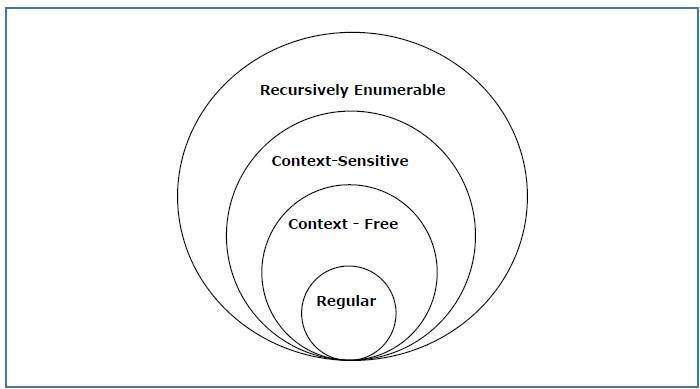
\includegraphics[ width=0.7\textwidth]{LinguaggiGerarchia}
	\caption[Gerarchia di linguaggi]{Gerarchia di linguaggi secondo Chomsky}
   \label{fig:linger}
\end{figure}
Ad una grammatica si può associare un unico linguaggio. Adesso si definirà come avvenie tale associazione:
\begin{definizione*}
Il linguaggio generato da una grammatica $\mathcal{G}$ è l'insieme di tutte le stringhe che possono essere derivate a partire dal simbolo iniziale S:\\

\centerline{$L(\mathcal{G}) = \{x \in \Sigma^{*} :S\xRightarrow[]{\mathcal{G}} x\}$}
\end{definizione*}
E' rilevante notare che come detto una grammatica genera un unico linguaggio ma un linguaggio può essere generato da molteplici grammatiche.\\
Inoltre la tassonomia di Chomsky non è esaustiva di tutti i linguaggi possibili, infatti esistono dei linguaggi che non sono ricorsivamente enumerabili cioè non c'è nessuna macchina di Turing che li riconosce.\\
Infine esistono altre classi di linguaggi che non sono incluse nella classificazione appena esposta e che saranno adoperate nel corso della trattazione:
\begin{definizione*}[Linguaggio Ricorsivo] Un linguaggio $L$ è detto \textbf{ricorsivo} se è decidibile cioè esiste una macchina di Turing $M$ che accetta ogni stringa in $x \in L$ e rigetta ogni stringa $x \not\in L$
\end{definizione*}
I linguaggi regolari e context-free sono ricorsivi. Esistono invece linguaggi context-sensitive non ricorsivi, cioè non ne sono un sottoinsieme \cite[p. 124]{Levelt08}. Tutti  i linguaggi ricorsivi sono ricorsivamente enumerabili (cioè sono anche linguaggi semidecidibili, per i quali una stringa non appartenente al linguaggio può essere sia rigettata che andare in ciclo infinito rispetto a una macchina di Turing) ma non è sempre vero il viceversa.
\begin{definizione*}[Linguaggio primitivo ricorsivo]
Un linguaggio è \textbf{primitivo ricorsivo} quando la sua funzione caratteristica è primitiva ricorsiva.
\end{definizione*}
Il concetto di funzione caratteristica è spiegato nella sezione \ref{sec:FSA}. Invece una funzione primitiva ricorsiva è una funzione definita come una delle funzioni di base o combinando le funzioni di base con operazioni come composizione e ricorsione. Per una definizione formale si rimanda a \cite{Rob47}. I linguaggi primitivi ricorsivi sono un sottoinsieme dei linguaggi ricorsivi.
\begin{definizione*}[Linguaggi superfiniti]
La classe dei linguaggi superfiniti è tale se contiene tutti i linguaggi finiti ed almeno un linguaggio infinito.
\end{definizione*}
 
\section{Automi a stati finiti}
\label{sec:FSA}
Nella sottosezione \ref{sub:gra} sono stati introdotti gli automi e una loro classificazione. Qui ci si concentrerà sullo studio dei \ac{FSA} in relazione ai linguaggi regolari, la classe dei linguaggi a cui questa tesi è rivolta. Come visto gli \ac{FSA} sono un caso speciale di \textit{macchina di Turing} e più nello specifico un caso speciale di \ac{FSM} che in questa sede non interessa definire. Qui basterà dire che   una \ac{FSM} è un \textit{transiction system} costituita da un insieme finito di stati dove ogni transizione è innescata da un'azione tra un insieme finito di azioni (di solito denotato da $\Sigma$). Esistono diversi tipi di \ac{FSM} come le \textit{Mealy Machines} e gli \ac{FSA}. Tra gli \ac{FSA} si annoverano gli \ac{NFA} strettamente correlati ai \ac{DFA} su cui si focalizzerà l'attenzione.
\begin{definizione}[Automa a stati finiti deterministico]
\label{def:dfa}
Un \ac{DFA} A è una quintupla:\\

\centerline{$A = \Braket{\Sigma,Q^{A},q_{\epsilon}^{A},\delta^{A}, \mathbb{F}_{\mathbb{A}}^{A}}$}
\end{definizione}
dove:\\
$\Sigma$ è un alfabeto\\
$Q^{A}$ è un insieme finito di stati\\
$q_{\epsilon}^{A} \in Q^{A}$ talvolta indicato come $q_{\lambda}^{A}$ è lo stato iniziale\\
$\delta^{A} : Q^{A} \times \Sigma \to Q^{A} $ è la funzione di transizione\\
$\mathbb{F}_{\mathbb{A}}^{A} \subseteq Q^{A}$ è l'insieme degli stati accettanti\\

Inoltre nel corso della trattazione seguendo \cite[p. 72]{DeLaHiguera10} in alcuni casi è conveniente utilizzare anche un'altra definizione per i \ac{DFA} uguale a quella appena data ma comprendente anche un nuovo insieme $\mathbb{F}_{\mathbb{R}}^{A} \subseteq Q^{A}$ che è l'insieme degli stati rigettanti. Quando si parlerà di \ac{DFA} si farà sempre riferimento alla prima definizione,quella classica,  a meno che non è specificato o l'utilizzo della seconda definizione risulta tacitamente evidente dall'utilizzo dell'insieme $\mathbb{F}_{\mathbb{R}}^{A}$. Si indica con $\norma{A} = \abs{Q^{A}}$. 
Inoltre in molti frangenti è conveniente utilizzare (questo è un discorso che esula dalla definizione di un \ac{DFA}) una versione estesa della funzione di transizione a una stringa anzichè ad un solo simbolo dell'alfabeto. Si definisce allora $\hat{\delta}^{A} : Q^{A} \times \Sigma^{*} \to Q^{A}$ definendo induttivamente $\hat{\delta}^{A}(q,\epsilon) = q \text{ e } \hat{\delta}^{A}(q,aw) = \hat{\delta}^{A}(\delta^{A}(q,a),w) \text{ per } q \in Q^{A} \text{ e } aw \in \Sigma^{+} \text{ e } w \in \Sigma^{*}$. Per la funzione di transizione estesa nel corso della tesi sarà anche usata interscambiabilmente la definizione $A[w] = \hat{\delta}^{A}(q_{\epsilon}^{A},w)$ . Inoltre si estende quest'ultima notazione agli insiemi di stringhe: $W \subseteq \Sigma^{*} \text{ | } A[W] = \{A[w] : w \in W\}$ .\\
 
Una stringa \textit{x} è detta essere accettata da un \ac{DFA} \textit{A} se e solo se $\hat{\delta}^{A}(q_\epsilon,x) = q'$ tale che $q' \in \mathbb{F}_\mathbb{A}^{A}$ che significa che usando la funzione di transizione estesa $\hat{\delta}^{A}$ a partire dallo stato iniziale è possibile arrivare ad uno stato accettante.   Il linguaggio individuato da un \ac{DFA} A è allora:\\
\centerline{$L(A) = \{x \in \Sigma^{*} : \hat{\delta}^{A}(q_\epsilon,x) \in \mathbb{F}_\mathbb{A}^{A}\}$}

Una relazione analoga a quanto visto tra linguaggi e grammatiche sussiste tra linguaggi e \ac{DFA}: un \ac{DFA} induce un solo linguaggio regolare, ma ad un linguaggio regolare corrispondono più \ac{DFA}.

In molti contesti è utile rifersi alla \textit{funzione di output}  di un \ac{DFA} A, $\lambda^{A}$ come:\\\\
\centerline{$
\lambda^{A} : \Sigma^{*} \to \mathbb{B}, \quad \forall w \in \Sigma^{*}\quad\lambda^{A}(w) = \begin{cases}
1
& \text{se $w \in L(A)$} \\
0 & \text{altrimenti}\\
\end{cases}
$}\\\\
La \textit{funzione di output} è la \textit{funzione caratteristica} di L(A).Inoltre $\lambda^{A}$ appena definita sopra può essere vista come un caso particolare, per $q=q_\epsilon^{A}$, di $\lambda_{q}^{A}(w)$ che assume valore  1 se $ \hat{\delta}^A(q,w) \in \mathbb{F}_{\mathbb{A}}^{A}$ . Ancora, due \ac{DFA} ,A e A' , sono \textbf{equivalenti} denotato da $A \cong A'$, se loro hanno la stessa \text{funzione di output}, cioè se $\lambda^{A} = \lambda^{A'}$, cioè se indivividuano lo stesso linguaggio. Il concetto di equivalenza è rilevante anche tra gli stati dello stesso \ac{DFA} ed informalmente due stati sono equivalenti se non esiste nessuna stringa che li distingue, cioè che partendo da quei due stati porta a stati di arrivo che sono uno accettante e l'altro no.
\begin{definizione*}[Stati equivalenti]
Detto A essere un \ac{DFA}, e q e p $\in Q^{A}$ stati di A. q e p sono \textit{equivalenti} ,denotato da $q \equiv p$, se $\lambda_{q}^{A} = \lambda_{p}^{A}$
\end{definizione*}
Una stretta correlazione tra l'equivalenza di stati e l'equivalenza di \ac{DFA} è il seguente risultato: $A \cong A' \Leftrightarrow q_{\epsilon}^{A} \equiv q_{\epsilon}^{A'}$.
Un altro concetto importante è quello di \textit{isomorfismo} tra due DFA.
\begin{definizione*}[Isomorfismo di \ac{DFA}]
Detti A ed $\text{A}'$ due \ac{DFA} definiti su $\Sigma$. A ed $\text{A}'$ sono detti isomorfici se esiste un isomorfismo $f : Q^{A} \to Q^{A'}$, cioè una funzione soddisfacente le seguenti condizioni:
\begin{enumerate}
\item $f(q_{\epsilon}^{A}) = q_{\epsilon}^{A'}$
\item $\forall q \in Q^{A} : q \in F_{\mathbb{A}}^{A} \Leftrightarrow f(q) \in F_{\mathbb{A}}^{A'}$
\item $\forall q \in Q^{A}, a \in \Sigma : f(\delta^{A}(q,a)) = \delta^{A'}(f(q),a)$
\end{enumerate} 
\end{definizione*}
L'isomorfismo è un requisito più forte dell'equivalenza: \ac{DFA} isomorfi sono pure equivalenti, ma in generale non è vero il contrario. Quindi dato un linguaggio L esistono più \ac{DFA} in grado di riconoscerlo cioè con la stessa \textit{funzione di output} $\lambda$. Tra questi di particolare interesse sono quelli con il minor numero di stati. Un \ac{DFA} A è detto \textbf{minimo} se qualunque altro \ac{DFA} $\text{A}'$ tale che $A \cong A'$ (con la stessa \textit{funzione di output}) soddisfa $\abs{Q^{A'}}\geq\abs{Q^{A}}$. Ovviamente in un \ac{DFA} minimo nè stati irragiungibili ne stati equivalenti possono essere presenti perchè potrebbero essere eliminati senza cambiare la funzione di output $\lambda$. Inoltre il DFA minimo è sempre unico a meno di una possibile rinomina degli stati. Per motivi storici esiste anche la definizione di \ac{DFA} \textbf{canonico} che è intercambiabile con quella di \ac{DFA} minimo ma entrambe indicano lo stesso ente matematico e sono del tutto equivalenti. Formalizzando
\begin{definizione*}[DFA minimo/canonico]
Detto A essere un \ac{DFA} su $\Sigma$. A è detto canonico se le seguenti condizioni sono verificate:
\begin{enumerate}
\item Tutti gli stati sono raggiungibili: $A[\Sigma^{*}] = Q^{A}$
\item Tutti gli stati sono a coppie separabili\footnote{due stati sono separabili o distinti se non sono equivalenti}: $\forall q \ne p \in Q^{A} : \exists w \in  \Sigma^{*} : \lambda_{q}^{A}(w) \ne \lambda_{p}^{A}(w)$
\end{enumerate}
\end{definizione*}
Per ogni DFA esiste sempre ,ed è unico (a meno delle etichette degli stati) un \ac{DFA} equivalente  che è canonico.
\subsection{FSA particolari}
Alcuni \ac{DFA} ed \ac{NFA} sono particolarmente significativi e ricorreranno spesso nell'ambito di questa tesi. Inoltre è necessario conoscere per il proseguio della trattazione qual è la differenza principale tra \ac{DFA} ed \ac{NFA}. Un \ac{NFA} è detto non deterministico perchè la sua funzione di transizione può avere più di una transizione per un dato simbolo dell'alfabeto (ed inoltre vi possono essere transizioni anche in corrispondenza di $\epsilon$). Inoltre in un \ac{NFA} non vi è necessariamente per ogni stato una transizione in corrispondenza di ogni simbolo dell'alfabeto.
\subsubsection{Maximal Canonical Automaton}
\begin{definizione}[Maximal Canonical Automaton]
Detto $I_+ = \{x_1,\cdots ,x_N\}$ un insieme di esempi positivi, si definisce \textit{\textbf{Maximal Canonical Automaton rispetto ad $I_+$}} e si denota con \textit{\textbf{MCA($I_+$)}} un \ac{NFA} costituito da una quintupla $\Braket{\Sigma , Q , q_\epsilon , \delta , \mathbb{F}_\mathbb{A}}$ dove:\\\\
$\Sigma$ è l'alfabeto su cui è definito $I_+$\\
$Q = \{q_{u}^{i} : u \in \text{Pref}(x_i) \land u \ne \epsilon \} \cup \{q_\epsilon\}, 1 \leq i \leq N$\\
$q_\epsilon = \{q_\epsilon\}$\\
$\delta(q_{u}^{i},a) = \{q_{ua}^{i} : ua \in \text{Pref}(x_i)\}, \forall a \in \Sigma, 1 \leq i \leq N$\\
$\delta(q_\epsilon,a) = \{q_{a}^{i} : a \in \text{Pref}(x_i)\}, \forall a \in \Sigma, 1 \leq i \leq N$\\
$1 \leq i \leq N, q_{x_{i}}^{i} \in \mathbb{F}_\mathbb{A} $\\
se $\epsilon \in I_+$ aggiungere $q_\epsilon \text{ ad } \mathbb{F}_\mathbb{A}$
\end{definizione}
Un \textit{MCA($I_+$)} per ogni stringa di $I_+$ ha un percorso dedicato a partire dallo stato iniziale.
Si noti che nella definizione data di $\delta$ accade che per molti simboli di $\Sigma$ non c'è la corrispondente transizione per un dato stato. Inoltre se in $I_+$ sono presenti stringhe che hanno lo stesso simbolo iniziale si avrà indeterminismo sullo stato iniziale $q_\epsilon$. Quindi in generale il \textit{MCA($I_+$)} è un \ac{NFA}.Un esempio è dato in figura \ref{fig:MCA}\\\\
\begin{figure}
\centering
\begin{tikzpicture}[shorten >=1pt,node distance=2cm,on grid,auto] 
   \node[state,initial] (q_0)   {$\varepsilon$}; 
   \node[state] (q_1) [above right=of q_0] {$a$}; 
   \node[state] (q_2) [below right=of q_0] {$a$}; 
   \node[state] (q_3) [right=of q_1] {$p$};
   \node[state,accepting] (q_4) [right=of q_3] {$e$};
   \node[state](q_5) [right=of q_2] {$t$};
   \node[state](q_6) [right=of q_5] {$o$};
    \node[state](q_7) [right=of q_6] {$l$};
    \node[state](q_8) [right=of q_7] {$l$};
    \node[state,accepting](q_9) [right=of q_8] {$o$};
    \path[->] 
    (q_0) edge  node {$a$} (q_1)
           edge  node {$a$} (q_2)
    (q_1) edge  node  {$p$} (q_3)
    (q_3) edge  node  {$e$} (q_4)
    (q_2) edge  node  {$t$} (q_5)
    (q_5) edge  node  {$o$} (q_6) 
    (q_6) edge  node  {$l$} (q_7)
    (q_7) edge  node  {$l$} (q_8) 
    (q_8) edge  node  {$o$} (q_9); 
\end{tikzpicture}
\caption[Maximal Canonical Automaton]{\textit{MCA($I_+$)} per $I_+=\{\text{ape,atollo}\}$}
\label{fig:MCA}
\end{figure}

\subsubsection{Automa quoziente}
\label{subsub:aqu}
Sia A un \ac{DFA} su $\Sigma$ e sia  $\approx \: \subseteq Q^{A}\!\!\times{}\!Q^{A}$ una relazione d'equivalenza sull'insieme $Q^{A}$ soddisfacente le seguenti due condizioni:
\begin{enumerate}[label=(\roman*)]
\item $\approx$ satura $\mathbb{F}_{\mathbb{A}}^{A}$
\item $\forall q,p \in Q^{A} : q \approx p \Rightarrow (\forall a \in \Sigma : \delta^{A}(q,a) \approx \delta^{A}(p,a) )$ 
\end{enumerate}
Allora da A tramite $\approx$ è possibile ricavare il \textit{\textbf{DFA quoziente}} \textbf{$A/\!\!\approx$} così definito:
\begin{enumerate}
\item $\Sigma$ è lo stesso di $A$
\item $Q^{A/\!\approx} = Q^{A}/\!\!\approx$
\item $q_\epsilon^{A/\!\approx} = [q_\epsilon^{A}]_\approx$
\item $\mathbb{F}_\mathbb{A}^{A/\!\approx} = \{[q]_\approx : q \in \mathbb{F}_\mathbb{A}^{A}\}$
\item $\delta^{A/\!\approx}([q]_\approx,a) = [\delta^{A}(q,a)]_\approx \quad \forall q \in Q^{A},a\in{\Sigma}$
\end{enumerate}
L'automa quoziente $A/\!\!\equiv$ ,dove la relazione d'equivalenza utilizzata è quella di equivalenza tra gli stati, corrisponde al \ac{DFA} canonico. Quindi banalizzando si può concludere dicendo che l'automa quoziente di un \ac{DFA} è ciò che si ottiene fondendo insieme alcuni stati del \ac{DFA} di partenza in base a una relazione d'equivalenza. Quando la relazione usata è quella di stati equivalenti si ottiene il DFA minimo: quindi $Q^{A/\!\approx}$ sarà una partizione in cui in ogni blocco (sottoinsieme) ci saranno stati equivalenti tra loro (in uno specifico blocco). Ogni blocco è una classe d'equivalenza.

\subsubsection{Prefix Tree Acceptor}
Si è visto che l'automa quoziente che si ottiene usando la relazione di equivalenza degli stati su un \ac{DFA} A è il \ac{DFA} minimo. Analogamente è possibile ottenere il \textit{\textbf{Prefix Tree Acceptor di $I_+$}} indicato con \textit{\textbf{PTA$(I_+)$}} applicando la definizione di automa quoziente al \textit{MCA$(I_+)$}\footnote{Anche se tecnicamente può essere un \ac{NFA} la definizione di automa quoziente può essere applicata comunque} con la relazione: \textit{stati che identificano lo stesso prefisso}. Quindi verrà effettuata la fusione degli stati che condividono lo stesso prefisso.\\
Si definisce la relazione d'equivalenza come:
\begin{equation*}
p \approx q \Leftrightarrow \text{ Prefix}(p) = \text{ Prefix}(q)
\end{equation*}
allora:
\begin{equation*}
MCA(I_+)/\!\!\approx \,\,=\, PTA(I_+)
\end{equation*}
In figura \ref{fig:PTA} il \textit{PTA} ricavato a partite dal \textit{MCA} di figura \ref{fig:MCA} .
\begin{figure}[htp]
\centering
\begin{tikzpicture}[shorten >=1pt,node distance=2cm,on grid,auto] 
   \node[state,initial] (q_0)   {$\varepsilon$}; 
   \node[state] (q_1) [right=of q_0] {$a$}; 
   \node[state] (q_3) [right=of q_1] {$p$};
   \node[state,accepting] (q_4) [right=of q_3] {$e$};
   \node[state](q_5) [below right=of q_1] {$t$};
   \node[state](q_6) [right=of q_5] {$o$};
    \node[state](q_7) [right=of q_6] {$l$};
    \node[state](q_8) [right=of q_7] {$l$};
    \node[state,accepting](q_9) [right=of q_8] {$o$};
    \path[->] 
    (q_0) edge  node {$a$} (q_1)
    (q_1) edge  node  {$p$} (q_3)
               edge  node  {$t$} (q_5)
    (q_3) edge  node  {$e$} (q_4)
    (q_5) edge  node  {$o$} (q_6) 
    (q_6) edge  node  {$l$} (q_7)
    (q_7) edge  node  {$l$} (q_8) 
    (q_8) edge  node  {$o$} (q_9); 
\end{tikzpicture}
\caption[Prefix Tre Acceptor]{\textit{PTA($I_+$)} per $I_+=\{\text{ape,atollo}\}$}
\label{fig:PTA}
\end{figure}

\subsubsection{Automa Universale}
Si indica con \textit{\textbf{UA l'automa universale}} che accetta tutte le stringhe definite su $\Sigma$. Si ha $L(UA) = \Sigma^{*}$. Ha un unico stato,che è accettante, con un \textit{self-loop} per ogni simbolo dell'alfabeto.

\subsection{Funzioni di output regolari}
In una sottosezione di \ref{subsub:aqu}  si è visto che è possibile ottenere il  \ac{DFA} canonico minimo di un \ac{DFA} A tramite $A/\!\!\equiv$ (l'automa quoziente sulla relazione di stati equivalenti). In questa sezione invece si vedrà come ottenere il \ac{DFA} canonico minimo non a partire da un \ac{DFA} preesistente, ma semplicemente sfruttando le proprietà di una funzione di output $\lambda : \Sigma^{*} \to \mathbb{B}$ che è la funzione caratteristica di qualche linguaggio regolare.
\subsubsection{Relazione di Nerode}
Si possono caratterizzare le \textit{funzioni di output regolare} come la classe di funzioni $\lambda : \Sigma^{*} \to \mathbb{B}$ per cui un \ac{DFA} con quella \textit{funzione di output} esiste\footnote{L'insieme delle funzione di output regolari identifica la classe dei linguaggi regolari}.  Il famoso teorema \textit{Myhill-Nerode} \cite{Ner58} fornisce una caratterizzazione alternative delle \textit{funzioni di output regolari} , che non fa affidamento sulla nozione di \ac{DFA}. Come primo step si definisce la \textit{relazione di Nerode} \cite{Ner58} sulle stringhe che definisce un'equivalenza sulle stringhe secondo $\lambda$:
\begin{definizione}[Relazione di Nerode]
\label{def:ner}
Sia $\lambda : \Sigma^{*} \to \mathbb{B}$ una funzione di output a due valori arbitraria definita su $\Sigma$. Due stringhe $u, u' \in \Sigma^{*}$ sono equivalenti secondo $\simeq_\lambda$\footnote{Si noti che per denotare l'equivalenza non si è usato il simbolo $\equiv$ (equivalenza tra stati) perchè qui si parla di equivalenza tra stringhe} denotato da $u \simeq_\lambda \!u'$ se e solo se:
\begin{equation*}
\forall v \in \Sigma^{*} \quad \lambda(uv) = \lambda(u'v)
\end{equation*}
dove $\simeq_\lambda \, \subseteq \Sigma^{*}\!\!\!\times\!\!\Sigma^{*}$ è una relazione binaria detta \textit{relazione di Nerode} o \textit{congruenza di Nerode} che definisce l'equivalenza tra stringhe secondo $\lambda$
\end{definizione}
\subsubsection{Teorema Myhill-Nerode}
La \textit{relazione di Nerode} $\simeq_\lambda$ può essere vista come l'equivalente a livello di stringhe della relazione di equivalenza $\equiv_A \subseteq Q^{A}\!\!\times\!Q^{A}$, sugli stati di un \ac{DFA} A. Dovrebbe essere osservato, tuttavia , che $\simeq_\lambda$ può essere definito per \textit{funzioni di output} arbitrarie, non solo regolari. Il teorema \textit{Myhill-Nerode}  fornisce una caratterizzazione delle \textit{funzioni di output regolari} basata su  $\simeq_\lambda$ :
\begin{teorema}[Teorema Myhill-Nerode o di caratterizzazione]
\label{teo:m-n}
Sia $\lambda : \Sigma^{*} \to \mathbb{B}$ una \textit{funzione di output} a due valori. $\lambda$ è regolare se e solo se la \textit{relazione di Nerode}  $\simeq_\lambda$ ha indice finito. 
\end{teorema}
Una dimostrazione del teorema si trova in \cite{Stef11}. L'implicazione in uno dei due versi del teorema dice che se $\simeq_\lambda$ ha indice finito, allora $\lambda$ è \textit{una funzione di output regolare} cioè esiste un \ac{DFA} A con $\lambda^{A} = \lambda$. Questo \ac{DFA} $A = \Braket{\Sigma,Q^{A},q_{\epsilon}^{A},\delta^{A},F_{\mathbb{A}}^{A}}$ è definito come:
\begin{itemize}
\item $\Sigma \text{ è il dominio di } \lambda$
\item $Q^{A} = \Sigma^{*}/\!\!\simeq_{\lambda}$
\item $q_{\epsilon}^{A} = [\epsilon]_{\simeq_{\lambda}}$
\item $F_{\mathbb{A}}^{A} = \{[u]_{\simeq_{\lambda}} | \: \lambda(u)=1\}$
\item $\delta^{A}([u]_{\simeq_{\lambda}} , a) = [u\!\cdot{}\!a]_{\simeq_{\lambda}}$ 
\end{itemize}
A è il \ac{DFA} minimo corrispondente al linguaggio identificato da $\lambda$.Si osservi come la costruzione del \ac{DFA} A è molto simile alla costruzione del \ac{DFA} minimo  usando la relazione di equivalenza sugli stati $\equiv$ usando l'automa quoziente a partire da un \ac{DFA}. Questo approccio alla costruzione degli automi è fondamentale nell'\textit{active learning}.

\chapter[Prel. e impl. ObP]{Preliminari e implementazione dell'Observation Pack}
\label{app:due}
Qui si presentano delle ulteriori notazioni inerenti prevalentemente il capitolo \ref{cap:quattro} e vengono svelati alcuni dettagli implementativi dell'\ac{ObP}.
\section{Notazione specifica per l'ObP}
In questo sezione vi è la delineazione di un'ulteriore notazione utilizzata principalmente nel capitolo \ref{cap:quattro} in congiunzione a quella introdotta in \ref{app:uno}, ma che essendo specifica dell'\ac{ObP} viene presentata in quest'appendice. Inoltre vi è anche la presentazione della notazione utilizzata per presentare un framework introdotto in \cite{StefCounterexample14} che facilità la compresione della correttezza e l'implentazione del metodo di gestione del controesempio in \ac{ObP}.
\subsection{Definizioni}
L'\ac{ObP} mantiene un insieme Sp,\textit{prefix-closed}, di \textbf{short prefix} detti anche \textbf{access sequence} ,che sono prefissi . Ogni short prefix identifica unicamente (cioè short prefix diversi identificano stati diversi in \ac{H} e nel target)  gli stati sia nel target A che nell'ipotesi \ac{H}. Ogni stato $q \in Q^{H}$ corrisponde unicamente ad una stringa (lo short prefix) $u \in Sp$, ed è assicurato che $H[u] = q$.  u è detta l'access sequence di q (in \ac{H}), ed è denotata da $\lfloor q \rfloor_{H}$ . Alternativamente quanto detto può essere formulato come $\forall q \in Q^{H} : \text{ \ac{H}}[\lfloor q \rfloor_{H}]=q$. Lo stato iniziale $q_{\epsilon}^{H}$ è lo stato con access sequence $\epsilon$.

Si estende questa notazione a stringhe arbitrarie $w \in \Sigma^{*} : \lfloor w \rfloor_{H} = \lfloor H[w] \rfloor_{H}$ che significa che w raggiunge uno stato in \ac{H} e questo stato ha un access sequence u cui w si associa. Quindi la funzione $\lfloor \cdot \rfloor_{H} : \Sigma^{*} \to Sp$ trasforma stringhe in access sequences.\\
Uno short prefix $u \in Sp$ corrisponde ad uno stato in A, cioè $A[u]$. Ci si riferisce ad $A[Sp]$ come gli stati scoperti (dal \textit{learner}) di A. Gli short prefixes quindi stabiliscono una funzione $f_{Sp}$ che collega stati nell'ipotesi e stati scoperti nel \ac{DFA} target A come segue:
\begin{equation*}
f_{Sp} : Q^{H} \to Q^{A} , f_{Sp}(q)=A[\lfloor q \rfloor_{H}]
\end{equation*}
\begin{comment}
Infine ,detto N l'insieme di nodi di un albero binario $\Upsilon$,si denota con o-child(n) la funzione d'utilità definita attraverso la funzione child(o,n) nella seguente maniera :
\begin{equation*}
\begin{multlined}
o-child=child : \mathbb{B} \times N  \to \{nil\} \cup N, \\
child(o,n)=\begin{cases}
n' & \parbox[t]{.6\textwidth}{se o=1 e n' è il figlio destro di n in $\Upsilon$ oppure o=0 e n' è il figlio sinistro di n in $\Upsilon$}\\
nil & \parbox[t]{.6\textwidth}{se o=1 e n non ha figli destri in $\Upsilon$ oppure o=0 e n non ha figli sinistri in $\Upsilon$}\\
\end{cases}
\end{multlined}
\end{equation*}
\end{comment}

%\thispagestyle{empty}

\subsection[Def. fram.]{Definizioni per il framework}
\label{sub:fra}
\subsubsection{Prefix Transformation}
\textit{Prefix transformation} è una procedura che consente di trasformare un prefisso di un controesempio $w \in \Sigma^{+}$ in un access sequence in Sp.
\begin{definizione*}[Prefix Transformation]
Prefix transformation rispetto ad \ac{H}, $\pi_{H}$ , è definita come segue:
\begin{equation*}
\pi_{H} : \Sigma^{*} \times \mathbb{N} \to \Sigma^{*} \text{ , } \pi_{H}(w,i) = \lfloor w_{[0,i)} \rfloor_{H} \cdot w_{[i,\abs{w})}
\end{equation*}
\end{definizione*}
Si osservi che, $\pi_{H}(w,0)=w \text{ e } \pi_{H}(w,\abs{w})=\lfloor w \rfloor_{H} \in Sp$.

\subsubsection{Altre definizioni}
Sia $w \in \Sigma^{+}$\footnote{In\ac{ObP} $\epsilon$ non può essere un controesempio} un controesempio che differenzia il target A da \ac{H}. Sia $m = \abs{w}$ ed i un indice $0\leq i \leq m$ allora si definisce la funzione $\alpha$ come:
\begin{equation*}
\alpha: [0,m+1) \to \mathbb{B}, \: \alpha(i) = \begin{cases}
1
& \text{se } \lambda^{A}(\pi_{H}(w,i)) = \lambda^{H}(w) \\
0 & \text{altrimenti}\\
\end{cases}\\\\
\end{equation*}
Dalla funzione $\alpha$ può essere ricavato anche la definizione della funzione $\beta$:
\begin{equation*}
\label{equ:beta}
\beta: [0,m) \to \{0,1,2\}, \: \beta(i) = \alpha(i) + \alpha(i+1)
\end{equation*}
\section[Dett. impl. ObP]{Dettagli implementativi dell' ObP}
\label{sec:implobp} 
Vengono ora riportati alcuni dettagli implementativi ritenuti più significativi senza pretesa di esaustività.
Per la memorizzazione della funzione OT (definizione \ref{def:obstable}) di un componente si è utilizzata una map che tipicamente è nella forma chiave-valore dove nella fattispecie la chiave è una stringa (ottenuta dalla concatenazione di un prefisso con un suffisso) ed il valore è l'esito delle \ac{MQ} nel target per quella stringa. Qui si è utilizzato per il valore un doppio campo, oltre all'esito della \ac{MQ} c'è un contatore che rappresena il numero di volte che quella stringa viene a formarsi in un dato componente (una stessa stringa può essere formata da  coppie prefisso-suffisso diverse). Questo è dovuto al fatto che quando si effettua uno split di un componente alcuni dei prefissi del componente migrano nei prefissi del nuovo componente. Oltre all'insieme dei prefissi del componente splittato (che va decrementato) si può modificare anche il dominio della funzione OT restringendolo. Nel codice si è scelto di eliminare la concatenazione del prefisso che migra nel nuovo componente con l'insieme di suffissi del componente splittato, restringendo il dominio di OT. Tuttavia per garantire la correttezza è necessario appurare se quella concatenazione di quel prefisso con un dato suffisso si venga a formare anche tramite altri prefissi perchè in questo caso l'eliminazione non deve avvenire ed è per questo motivo che si usa un contatore per ogni stringa (per ogni concatenazione) che va incrementato ad ogni inserimento di una stringa (anche una già esistente) e decrementato nel caso suddetto.  Questa scelta è stata fatta nell'ottica di consentire velocemente di appurare se un componente è chiuso e in generale consentire una ricerca molto veloce di un prefisso in un componente. L'alternativa sarebbe stata quella di non utilizzare il contatore e non eliminare mai la stringa formata dalla concatenazione di un prefisso e di un suffisso ma solo il prefisso dal componente splittato. Ciò porterebbe ad una crescita del dominio di ricerca per la funzione OT che degraderebbe le prestazioni della ricerca di un prefisso in un componente (operazione effettuata sovente) anche se potrebbe  comportare una diminuizione del numero delle \ac{MQ} e l'eliminazione dell'\textit{overhead} per tenere aggiornato il contatore: questa prospettata diminuizione delle \ac{MQ} con questa seconda scelta è però possibile soltanto se quando si completano le componenti, ad esempio nella funzione UPDATE-FROM-COUNTEREXAMPLE  prima di effettuare una \ac{MQ} su una stringa x si controlli se per x non si conosca già l'esito della \ac{MQ} perchè contenuto già nel dominio della funzione OT\footnote{più è grande il dominio e maggiore sarà la probabilità di ottenere un \textit{hit} per x} anche se nel caso vi fossero molti \textit{miss} questa politica potrebbe essere addirittura controproducente. Anche quest'ulteriore strategia non è stata implementata ritenendo poco probabile un \textit{hit} (per implementarla basta decommentare un if  in UPDATE-FROM-COUNTEREXAMPLE e aggiungerne un altro nella funzione \textit{sift}). Se si fossero fatte delle scelte opposte a quelle fatte e appena descritte senz altro si sarebbe potuto abbassare ulteriormente il numero di \ac{MQ} ma si è ritenuto che il gioco non vale la candela cioè che il prezzo da pagare in termini di tempo di esecuzione per ottenere ciò è maggiore del beneficio ottenuto.\\
Si sottolinea che diversamente dal metodo OBP-SPLIT (algoritmo \ref{alg:split}) non viene ritornato il nuovo componente ottenuto perchè il chiamante OBP-CLOSEPACK ne è già a conoscenza , quindi il metodo non ritorna niente.\\
Infine si prende in esame l'implementazione del discrimination tree. Per quest ultimo si è scelto di usare un \textit{vector} di nodi e un insieme di archi. Per ogni nodo si memorizza l'etichetta e se è accettante o meno. Gli archi sono un \textit{vector} di array bidimensionali. L' indice di un nodo nel \textit{vector} di nodi è usato per accedere alla posizione nel \textit{vector} di archi che contiene gli indici dei nodi figli (nell'array contenuto nel \textit{vector} di nodi nella posizione individuata dall'indice del nodo). L'utilizzo di un insieme di nodi e di archi è tipico di un grafo piuttosto che di un albero binario. Si è scelta ugualmente questa implementazione essenzialmente per due ragioni:
\begin{itemize}
\item La \textit{Standard Template Library} non mette a disposizione nessuna struttura dati per modellare una albero binario. Esistono delle librerie esterne che mettono a disposizioni un albero n-ario ma l'overhead per gestire n figli ed altre operazioni inutili ai fini dell'\ac{ObP} ha fatto propendere per il declinare il loro utilizzo. Un'altra possibilità sarebbe stata quella d'implementare un albero binario \textit{ad hoc} nella maniera classica cioè tramite i puntatori ma essendo le prestazioni simili a quelle della soluzione adottata e descritta sopra non lo si è fatto. Inoltre si è supposto che chiamare un oggetto di una classe esterna (quella dell'eventuale implementazione dell'albero binario), dato che va fatto molte volte, sarebbe divenuto il costo preponderante. Il vantaggio principale nell'usare l'implementazione di un albero binario con i puntatori per il discrimination tree sta nel risparmio di memoria circa doppia ma comunque sempre lineare nella soluzione proposta, e che non avviene mai la riallocazione (operazione che accade quando le dimensioni del vettore superano la capacità dello stesso).
\item Utilizzare un vettore indicizzato. Questa soluzione è da scartare perchè se il discrimination tree non è bilanciato e presenta un ramo molto più lungo degli altri sarebbe necessario rendere il vettore molto grande. Il vettore può crescere dinamicamente ed è molto più probabile con un vettore indicizzato superare la capacità totale del vettore (se l'inserimento del nodo avviene nello stesso ramo ciò avviene molto velocemente) che verrebbe quindi riallocato e ricopiato frequentemente degradando le prestazioni.
\end{itemize} 
 
 
 
 
 
 
 
 \chapter{SVM} 
\label{cap:cinque}
La tesi è volta ad investigare lo scenario in cui si utilizzi un classificatore come base per costruire un Oracolo. Da quest esigenza nasce la necessità di utilizzare uno dei tradizionali metodi statistici di \textit{machine learning}. Nella fattispecie si deve risolvere un problema di \textbf{classificazione binaria} dato che il modello, una volta avvenuto l'addestramento, ha lo scopo di predire come accettante o rigettante , cioè appartenente o meno ad \ac{L} , il campione sotto esame.\\
Tra i moltissimi metodi statistici esistenti forse i più noti sono \textit{Random Forest, Recurrent Neural Network, Convolutional Neural Network} e \ac{SVM}. Tra questi un metodo che è stato molto utilizzato nell'apprendimento di linguaggi è una riadattazione delle \textit{Reti Neurali Ricorrenti}, che si sono dimostrate adeguate allo scopo. In queste sede si è scelto di usare le \ac{SVM} perchè rappresentano un classificatore molto potente, e sebbene esistano dei lavori inerenti il tema \cite{Kontorovich09} non sono stati contestualizzati nell'ambito dell'\textit{active learning} per \ac{IIR} oppure sono limitati all'apprendimento di alcune specifiche classi di linguaggi \cite{Cortes08} \cite{Clark06} \cite{Clark11}.

\section{Overview teorica}
Il problema che si tenta di risolvere con le \ac{SVM} , che è la radice da cui nascono anche altri modelli , appare sotto diversi nomi come il compromesso bias-varianza, controllo della capacità e dell'\textit{overfitting} dei dati, ma l'idea è la stessa: dato un problema di \textbf{apprendimento supervisionato}, cioè con un insieme di addestramento di cardinalità finita che contiene i dati etichettati con la rispettiva classe di appartenenza (il \textit{training set}) , le migliori \textit{performances} di generalizzazione\footnote{Cioè una migliore capacità di predire correttamente la classe di appartenenza di dati mai visti, cioè non contenuti nel \textit{training set}. Per questo motivo si parla di classificazione.} del classificatore saranno ottenute dal raggiungimento del giusto equilibrio tra l'\textit{accuracy} sul training set del classificatore e la capacità del modello. La capacità di un modello di classificazione statistico rappresenta la complessità, la potenza espressiva, la ricchezza piuttosto che la flessibilità della famiglia di funzioni $f(x,\alpha)$:
\begin{equation*}
\label{eq:effe}
f : X \to Y \quad \text{con } X=\{x_{1},x_{2},\dots,x_{l}\} 
\end{equation*}
$X$ contiene i campioni e rappresenta il \textit{training set} e $Y$ rappresenta i possibili valori delle etichette di ciascun campione e nel caso di \textbf{classificazione binaria} $Y=\{0,1\}$. Inoltre si parla di famiglia di funzioni perchè \ac{SVM} (come gli altri modelli) ha una serie di iperparametri ,rappresentati da $\alpha$ , che identificano i diversi classificatori\footnote{Classificatore e modello non sono termini interscambiabili. Il modello è rappresentato dalle funzioni $f(x,\alpha)$ con $\alpha$ generico ,un classificatore invece è una singola funzione che si ottiene dal modello per una specifica istanza degli \textit{iperparametri} $\alpha$.}.  Una capacità alta implica che le funzioni $f(x,\alpha)$ sono complesse cioè di alto grado ad esempio: il discorso è analogo a ciò che accade in una feedback-forward con tante unità nascoste. Per il principio del \textit{Rasoio di Occam} (sezione \ref{sec:limIIR}) è bene selezionare il classificatore con la capacità minima che contemporaneamente si adatta ai dati del \textit{training set} ma come si vedrà i due aspetti sono in contrapposizione e sarà necessario trovarne il giusto compromesso. Questo assunto più avanti sarà approfondito e giustificato. Per il momento basti dire che un classificatore con troppa capacità è come un botanista con una memoria fotografica che quando vede un albero mai visto --- cioè appartenente a quello che formalmente viene identificato come \textit{test set} --- conclude che non è un albero perchè ha un numero di foglie diverso dagli alberi visti finora: situazione detta di \textit{overfitting} in cui il classificatore si è adattato esclusivamente ai dati del \textit{training set} ma non generalizza (analogo della rete neurale con troppe unità nascoste rispetto alla cardinalità del \textit{training set}). D'altro canto una macchina con bassa capacità è come il fratello pigro del botanista  che classifica qualunque cosa sia verde come un albero. In nessuno dei due casi si avrà una buona generalizzazione.

\subsection{Rischio Atteso}
Supponiamo di avere $l$ osservazioni nel \textit{training set}. Ogni osservazione è una coppia: un vettore $x_{i} \in \mathbb{R}^{n} \text{ , } i=1,\cdots,l$ e l'etichetta corretta  associata $y_{i}$. Per semplicità $y_{i} \in \{-1,1\}$. Si assume che le coppie $(x_i,y_i)$ siano estratte da una distribuzione di probabilità cumulativa (CDF) che si indica con $P(x,y)$,  e con $p(x,y)$ la corrispondente densità di probabilità (PDF).  Supponiamo che il modello sta provando ad imparare il mapping $x_i \to y_i \text{ per } i=1,\dots,l$.  Il modello è definito da una serie di possibili mapping $f(x,\alpha) \text{ tali che } x \to f(x,\alpha) $. Il modello rappresenta la classe di funzioni $f(x,\alpha) $, si parla di classe perchè più funzioni possono essere imparate dal modello cambiando gli \textit{iperparametri} $\alpha$.  Fissare gli $\alpha$ (che possono essere più di uno) per un modello si concretizza in un modello ``trained'', cioè in uno specifico classificatore. Ad esempio se il modello è una rete neurale gli \textit{iperparametri} $\alpha$ sono tipicamente i pesi e il bias. \\ Seguendo il riferimento \cite{Vapnik95}, si può definire il \textbf{rischio atteso} per un classificatore ($\alpha$ fissato) come:
\begin{equation}
\label{eqn:rischioatteso}
R(\alpha) = \int \frac{1}{2} \abs{y-f(x,\alpha)} \, dP(x,y) = \int \frac{1}{2} \abs{y-f(x,\alpha)} \, p(x,y) \, dx \, dy
\end{equation}
Il rischio atteso è anche detto \textbf{true mean error}  dato che è calcolato su tutti i possibili valori di $x$ e $y$ ($X \times Y$) cioè tiene conto di tutte le combinazioni sia sulle coppie nel \textit{training set} sia di tutte quelle mai osservate. Inoltre nell'equazione \eqref{eqn:rischioatteso}  $1/2 \abs{y-f(x,\alpha)}$ è una \textbf{funzione di loss} , ma se ne poteva scegliere un'altra infatti in generale si ha $V(f(x,\alpha),y)$. La specifica funzione di loss scelta nell'equazione \eqref{eqn:rischioatteso} può assumere solo valori in $\mathbb{B}$. Tuttavia $R(\alpha)$ così definito non è utile in quanto quasi mai si conosce $P(x,y)$ o una sua stima ,allora si definisce il \textbf{rischio empirico} per un classificatore:
\begin{equation*}
R_{emp}(\alpha) = \frac{1}{2l} \sum_{i=1}^{l}\abs{y-f(x_{i},\alpha)}
\end{equation*}
e rappresenta il tasso di errore medio sul \textit{training set}. $R(\alpha) - R_{emp}(\alpha)$ è l'errore di generalizzazione. Si dice che un modello generalizza se
\begin{equation*}
\lim_{ l \to \infty} R(\alpha) - R_{emp}(\alpha) = 0
\end{equation*}   
cioè al crescere degli elementi nel \textit{training set} gli elementi mal predetti nel \textit{test set} diminuiscono. Ma come già detto il rischio atteso non è quasi mai calcolabile per come è stato definito, allora con un'impostazione molto simile al \textit{PAC-learning} introdotto in \ref{def:PacL} Vapnik ha dimostrato in \cite{Vapnik95}  che:

\begin{align}
  \intertext{Definiti} 
  \eta &\text{ : } 0 \leq \eta \leq 1 \notag \\ 
  h &\text{ : } h > 0 \\
  \upvarepsilon &= \sqrt{\biggl(\frac{h(\log (2l/h) + 1) - \log (\eta/4)}{l}\biggl)}\\ \intertext{allora si ha che:} 
  R&(\alpha) \leq R_{emp}(\alpha) +\upvarepsilon \quad \text{con probabilità }1-\eta \label{eqn:vapnik}
\end{align}

dove $h$ è detta \ac{VC} \textbf{dimension} e $\upvarepsilon$ è detto \textbf{learning rate} o \textbf{\ac{VC}} \textbf{\textit{confidence}}. La \ac{VC} \textit{dimension} è una misura della capacità e sarà approfondita nella sottosezione \ref{sub:vcdim}.  $R_{emp}(\alpha) +\upvarepsilon$ è talvolta detto \textbf{\textit{risk bound}} dato che è un limite superiore del rischio atteso $R(\alpha)$.  Il risultato dell'equazione \eqref{eqn:vapnik} ci consente di trovare con probabilità $1-\eta$ il classificatore che minimizza $R_{emp}(\alpha) +\upvarepsilon$. Tuttavia calcolare questo minimo è molto difficile come è spiegato nella sottosezione \ref{sub:srm}. Prima di parlarne si spiega cosa è la \ac{VC} \textit{dimension}.

\subsection{\textit{VC dimension}}
\label{sub:vcdim}
La \ac{VC} \textit{dimension} è una misura della capacità di un insieme di funzioni $\{f(x,\alpha)\}$ che possono essere apprese da un modello statistico, ed è definita come la cardinalità del più largo insieme di punti che un modello può \textbf{\textit{shatter}}. Per \textit{shatter} si intende che una delle funzioni è in grado di etichettare correttamente i punti o meglio di separare punti (che sarebbero dei campioni, delle osservature) con etichettature diverse. Ci si pone  nel caso della classificazione binaria e si fissa il codominio di $\{f(x,\alpha)\}$  in $\{-1,1\} \forall x,\alpha$.  Se un insieme $X$ di $l$ punti viene etichettato in tutti i $2^l$ possibili modi, e per ognuna delle $2^l$ combinazioni, può essere trovata una funzione (con $\alpha$ specifico cioè un classificatore) dell'insieme $\{f(x,\alpha)\}$ che separa (o assegna) correttamente queste etichette, si dice che l'insieme di punti $X$ è ``\textit{shattered}'' dall'insieme di funzioni. Quindi la \ac{VC} \textit{dimension} dell'insieme di funzioni $\{f(x,\alpha)\}$ è definita come il \textbf{massimo} numero di punti che possono essere ``\textit{shattered}'' da $\{f(x,\alpha)\}$. Si osservi che avere per esempio una \ac{VC} \textit{dimension}  pari a tre significa che esiste almeno un insieme fatto da tre punti che può essere ``\textit{shattered}'', ma non è detto (tipicamente non lo è) che tutti gli insiemi di tre punti lo siano\footnote{In questo caso si può solo concludere che non esiste nessun insieme di quattro punti che è ``\textit{shattered}''}. Si fornisce come esempio il calcolo delle \ac{VC} \textit{dimension} dell'insieme costituito da tutte le rette in $\mathbb{R}^2$ identificate dall'equazione $y = mx + q$ in cui i parametri $\alpha$ sono rappresentati da $m \text{ e } q$. I punti possono essere etichettati positivamente o negativamente, quindi per essere ``\textit{shattered}'' da una retta devono essere separati da quest'ultima in base all'etichettatura. Inoltre si rimarca che i punti possono essere collocati in qualunque maniera, ma una volta collocati le varie etichettature devono essere effettuate mantenendo fissa quella collocazione scelta. Con tre punti, si riesce a trovare una collocazione dei tre punti (qualsiasi tranne tre punti allineati) tale che esiste una retta (valori specifici di $m$ e $q$)  che separari i punti positivi da quelli negativi e si riesce a fare ciò per ciascuna delle $2^{3}=8$ etichettature diverse\footnote{Si noti che in queste 8 etichettature  la collocazione dei 3 punti deve restare costante ma si può scegliere un'altra funzione (retta) da un'etichettatura all'altra} come si può apprezzare in figura \ref{fig:sha}. 
\begin{figure}[htp]
	\centering
	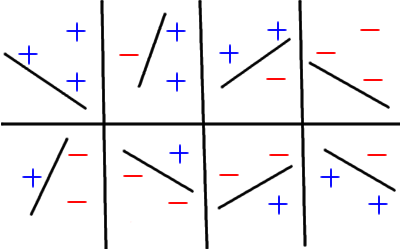
\includegraphics[ width=0.7\textwidth]{RettaShatter}
	\caption[Tre punti shattered nel piano]{Tre punti in $\mathbb{R}^{2}$ , shattered da rette}
   \label{fig:sha}
\end{figure} 

Quattro punti non possono essere ``\textit{shattered}'' quindi la \ac{VC} \textit{dimension} è tre. Più in generale la \ac{VC} \textit{dimension} dell'insieme di iperpiani in $\mathbb{R}^{n}$ è $n+1$. Una dimostrazione di questo risultato si può trovare in \cite[p. 37]{Burges98}. 

\subsection{Structural Risk Minimization}
\label{sub:srm}
La \ac{VC} \textit{dimension} di un modello riveste un ruolo molto importante perchè come si evince dai risultati dell'equazione  \eqref{eqn:vapnik}  ,fissati $\eta \text{ e } l$, si ha che la \ac{VC} \textit{confidence} $\upvarepsilon$ aumenta all'aumentare della \ac{VC} \textit{dimension} $h$. Quindi per diminuire il rischio atteso $R(\alpha)$ sembra sufficiente diminuire $h$ ma in realtà non è così. 
Innanzitutto si precisa che un numero di parametri ($\alpha$) maggiore nel modello non implica  una \ac{VC} \textit{dimension} maggiore infatti esistono dei modelli con un solo parametro e \ac{VC} \textit{dimension} infinita. Inoltre possedere un valore di $h$ più piccolo non comporta necessariamente di avere un rischio atteso più piccolo e quindi un classificatore migliore infatti un valore di $h$ più piccolo significa che è stato ristretto l'insieme delle funzioni $\{f(x,\alpha)\}$ e può accadere che è stata eliminata proprio la funzione che minimizzava il rischio empirico. Quindi dinimuendo $h$ la \ac{VC} \textit{confidence} $\upvarepsilon$ diminuisce ma il rischio empirico può aumentare e quindi diminuire $h$ non implica che il rischio atteso $R(\alpha)$ diminuisca\footnote{Esistono modelli che hanno buoni riscontri pratici nonostante abbiano $h = \infty$}. Il motivo di questo comportamento è che la \ac{VC} \textit{confidence} dipende dalla classe di funzioni $\{f(x,\alpha)\}$ invece il rischio empirico dipende dalla scelta degli \textit{iperparametri} e quindi da una specifica funzione. \\ Al fine di minimizzare $R(\alpha)$ si deve trovare il giusto compromesso tra due quantità che manifestano un andamento opposto al variare di $h$: il rischio empirico (che diminuisce all' aumentare della complessità di  $\{f(x,\alpha)\}$ cioè della capacità del modello cioè all'aumentare di $h$) e la \ac{VC} \textit{confidence} (che diminuisce al diminuire di $h$). Vapnik in \cite{Vapnik82} ha proposto una procedura per affrontare il problema appena delineato detta \ac{SRM} che consiste nel:
\begin{enumerate}
\item Dividere la famiglia di funzioni $\{f(x,\alpha)\}$ in sottoinsiemi autoincludenti come in figura \ref{fig:ssrm} in modo che i sottoinsiemi abbiano una \ac{VC} \textit{dimension} (che è un valore intero) crescente. Ciò significa escludere alcune funzioni da $\{f(x,\alpha)\}$ in modo da trovare la classe di funzioni $h_1$ con \ac{VC} \textit{dimension}  più piccola e così via per $h_{2} \text{,}h_{3}\dots$

\item Per ogni classe di funzioni trovate al punto 1. ($h_{1} \text{,}h_{2}\dots$) trovare quella con il rischio empirico minimo: cioè equivale a una selezione dei parametri. Ad esempio per la classe $h_1$ significa trovare la funzione contenuta in $\{h_{1}(x,\alpha)\}$ che minimizza il rischio empirico (ciè equivale a trovare i parametri $\alpha$ che fanno ciò).

\item Selezionare il classificatore tra quelli trovati al punto 2. che minimizza $R(\alpha)$
\end{enumerate}

\ac{SRM} garantisce un compromesso tra la qualità dell'approssimazione dei dati nel \textit{training set} e la complessità della funzione approssimante come illustrato in figura \ref{fig:srm}

\begin{figure}[htp]
	\centering
	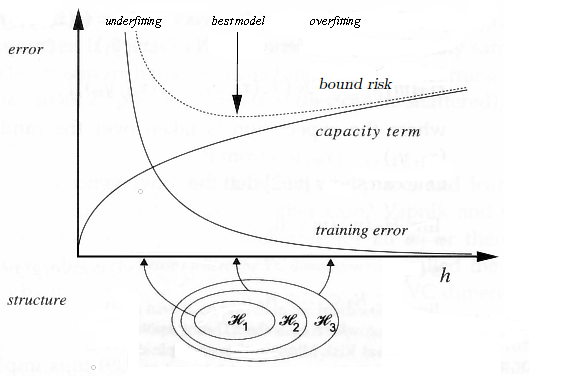
\includegraphics[ width=0.7\textwidth]{SRM}
	\caption[Principio della SRM]{Il \textit{risk bound} è la somma del rischio empirico e la \ac{VC} \textit{confidence}. Il più piccolo \textit{risk bound} è raggiunto su qualche elemento della struttura. }
   \label{fig:srm}
\end{figure} 

\ac{SRM} non è quasi mai applicabile perchè è molto complicato riuscire a calcolare la \ac{VC} \textit{dimension}  delle ``sottofunzioni'' e anche se ciò fosse possibile la difficoltà computazionale per calcolare il rischio empirico , a causa della spesso grande dimensionalità dello spazio degli \textit{iperparametri} del modello, è insostenibile. Si vedrà nelle sottosezioni \ref{subsub:lsrm} e \ref{subsub:srmsoft} che il principio di funzionamento delle \ac{SVM} ricalca concettualmente  da vicino quello della \ac{SRM}.

 \begin{figure}[htp]
	\centering
	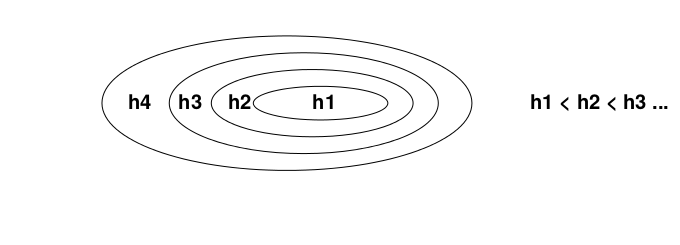
\includegraphics[ width=0.7\textwidth]{SottoinsiemiSRM}
	\caption[Sottoinsiemi SRM]{Famiglia di funzioni del modello suddivise in base alla \ac{VC} \textit{dimension} }
   \label{fig:ssrm}
\end{figure}

\section{SVM}
Le Support Vector Machines (\ac{SVM}) sono un metodo d'apprendimento supervisionato, introdotte per la prima volta da Vapnik e Chervonenkis nel 1963. Nel corso degli anni sono state introdotte varie versioni di \ac{SVM} tra cui ne sono rimarcabili quattro:
\begin{enumerate}
\item Quella originale: Il \textit{Maximal Margin Classifier}.
\item La versione con il \textbf{\textit{kernel}}.
\item La versione detta \textbf{\textit{soft-margin}}.
\item La versione \textit{soft-margin} con \textit{kernel} che combina i tre punti precedenti.
\end{enumerate}
La letteratura sull'argomento è sterminata e \cite{Osuna97} \cite{Burges98} \cite{Ng}  sono solo alcuni dei riferimenti esistenti. Da essi si è tratto gran parte del materiale presentato in questa sezione.
 Le \ac{SVM} consentono di affrontare essenzialmente tre tipi di problemi:
\begin{itemize}
\item Classificazione binaria
\item Classificazione con più classi
\item Regressione lineare
\end{itemize}   

La classificazione binaria è naturale con \ac{SVM} ed è adatta a quei problemi in cui i dati possono appartenere a due classi distinte (etichettate di solito con 1 o -1).\\
Nella classificazione con più classi i dati possono appartenere a più classi.
Nella regressione lineare lo scopo è determinare una funzione lineare che meglio approssimi  un insieme di dati.\\
Il problema affrontato in questa tesi attiene ai problemi di classificazione binaria.

\subsection{Classificazione binaria}
\label{sub:clb}
Un problema di classificazione per molti versi è simile a un problema di inferenza induttiva (capitolo \ref{cap:uno}). Da una serie di osservazioni cioè di elementi del \textit{training set} X si deve estrarre il migliore classificatore dallo spazio delle ipotesi $f(x,\alpha)$ secondo qualche criterio di preferenza. Gli elementi del training set in un problema di classificazione binaria supervisionato sono del tipo $(x_i , y_i)$ con $i=1,\dots,l$ cioè $\abs{X}=l$ , $x_i \in \mathbb{R}^{n}$ cioè ogni singolo elemento del \textit{training set} ha dimensionalità $n$, e $y_i \in Y=\{-1,1\}$ (o $\mathbb{B}$ in alcuni casi). La dicotomia delle etichette dell'insieme $Y$ rende la classificazione di tipo \textit{binaria}.
 Nel caso delle \ac{SVM} le funzioni sono del tipo:
\begin{equation*}
f : X \subseteq \mathbb{R}^{n} \to \mathbb{R}
\end{equation*}
Da un punto di vista geometrico la classificazione binaria nelle \ac{SVM} consiste nel trovare l' iperpiano ottimo ,secondo qualche criterio, nello spazio $\mathbb{R}^n$  che separi i dati del \textit{training set} etichettati positivamente da quelli etichettati negativamente. Se almeno un iperpiano siffatto esiste i dati del \textit{training set} sono detti essere \textbf{linearmente separabili}. Un esempio in figura \ref{fig:lsd}\\
Da un punto di vista analitico è necessario una funzione lineare che classifichi correttamente il \textit{training set}. Una funzione lineare,cioè un iperpiano,  è nella forma:
\begin{equation*}
f(x) = w \bullet x +b = \Biggl(\sum_{i=1}^{n}w_{i}x_{i}\Biggl) + b
\end{equation*}
Quindi la dipendenza dai parametri $\alpha$ si riconduce alla dipendenza da $w$ --- che è un vettore nello spazio $\mathbb{R}^n$ che rappresenta la normale all'iperpiano --- e $b$ uno scalare che consente all'iperpiano di muoversi parallelamente a se stesso.\\  
Una volta scelto il classificatore dallo spazio delle ipotesi, l'ingresso $x=(x_1,x_2,\dots,x_n) $ del \textit{test set} (cioè di un insieme di elementi non sottoposti in fase di addestramento al modello) sarà classificato in base all'esito della funzione $sign(f(x))$ cioè associato alla classe positiva se $f(x) \geq 0$, altrimenti sarà associato alla classe negativa.
 
 \begin{figure}[htp]
	\centering
	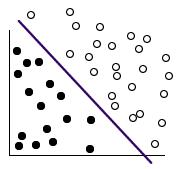
\includegraphics[ width=0.5\textwidth]{linearlyseparabledata}
	\caption[Lineare separabilità]{Dati in $\mathbb{R}^{2}$ linearmente separabili}
   \label{fig:lsd}
\end{figure}

\subsection{Classificatore  a margine massimo}
\label{sub:cmm}
Il \textit{Maximal Margin Classifier} rappresenta la versione iniziale di \ac{SVM} e spesso in letteratura questa tecnica è nota anche come \textbf{hard margin}. Si applica quando i dati sono \textbf{linearmente separabili}. Come accennato nella sottosezione \ref{sub:clb} è necessario trovare il ``migliore'' iperpiano che separa linearmente i dati nel \textit{training set}. Ai nostri scopi per lineare separabilità si intende che si può trovare una coppia $(w,b)$ tale che i seguenti vincoli sono rispettati:
\begin{align*}
&w \bullet x_i + b \geq \:\:\:1 \quad \quad \qquad\text{ per } y_i = +1 \:\:\:\forall i\\
&w \bullet x_i + b \leq -1 \quad \quad \qquad\text{ per } y_i = -1 \:\:\:\forall i
\end{align*}
I due vincoli possono essere convenientemente combinati insieme in modo da ottenere un unico vincolo più compatto:
\begin{equation}
\label{eq:vin}
y_i(w \bullet x_i + b) - 1 \geq 0 \qquad \qquad \forall i
\end{equation}
Il vincolo \eqref{eq:vin}  deriva dalla constatazione che la \textit{\textbf{decision function}} $sign(w \bullet x + b)$, cioè l'iperpiano separatore ,rispettante il vincolo \eqref{eq:vin}, che viene selezionato come migliore , è tale che se $w$ e $b$ sono scalati\footnote{Per scalati si intende moltiplicati} per la stessa quantità scalare $\alpha \in \mathbb{R}^{+}$  il vincolo \eqref{eq:vin} è ancora rispettato. Dunque per eliminare questa ridondanza , e per rendere ogni \textit{decision function} corrispondente ad un'unica coppia $(w,b)$, viene imposto il seguente vincolo:
\begin{equation}
\label{eq:vin2}
\min_{i=1,\dots,l}^{}\abs{w \bullet x_{i} + b} = 1
\end{equation}
che è un modo equivalente di scrivere il vincolo \eqref{eq:vin}.  Nel gergo tecnico delle \ac{SVM} si suole dire che si è scelto un parametro $\alpha$ tale che il \textit{margine funzionale dell'iperpiano}\footnote{Informalmente il \textit{margine funzionale dell'iperpiano} è la distanza minima tra tutti i punti del \textit{training set} e l'iperpiano separatore} è pari a 1 cioè la valutazione della \textit{\textbf{decision function}} nei punti del \textit{training set}  più vicini all'iperpiano separatore è tale che\footnote{Si può dimostrare che l'esistenza di tali punti è assicurata}
\begin{align}
&w \bullet x_i + b = \:\:\:1 \qquad \qquad\text{ per } y_i = +1 \label{eqn:h1}\\
&w \bullet x_i + b = -1 \qquad \qquad\text{ per } y_i = -1  \label{eqn:h2}
\end{align}
L'nsieme di iperpiani che soddisfano \eqref{eq:vin} sono detti \textbf{Iperpiani Canonici}\footnote{In molte trattazioni si definisce il margine geometrico come il margine funzionale rispetto all'iperpiano normalizzato rispetto a $\norma{w}$ e poi si dimostra che margine funzionale e margine geometrico coincidono imponendo il vincolo  \eqref{eq:vin}}.  Per un'\textit{iperpiano canonico} in cui il margine geometrico e il \textit{margine funzionale dell'iperpiano} coincidono si può dare una definizione intuitiva di \textbf{margine}.
\begin{definizione}
\label{def:mar}
Si indichi con $d_+$ la più breve distanza dell'iperpiano separatore dal più vicino esempio positivo del \textit{training set} e con $d_{-}$ la più breve distanza dall'esempio negativo più vicino del \textit{training set}. Allora:
\begin{equation*}
margine = d_{+} + d_{-}
\end{equation*}
\end{definizione}

Si può dimostrare che la distanza di un generico punto $x$ da un iperpiano $w \bullet x +b$ è pari a:
\begin{equation*}
d = \frac{\abs{w \bullet x + b}}{\norma{w}}
\end{equation*}
In accordo alla normalizzazione definita in \ref{eq:vin2} la distanza tra l'\textit{iperpiano canonico} e il più vicino degli elementi del \textit{training set} è $\frac{1}{\norma{w}}$. Quindi il margine di un \textit{iperpiano separatore canonico} secondo la definizione \ref{def:mar} è allora $\frac{2}{\norma{w}}$. L'immagine  \ref{fig:lsdmar} può essere chiarificatrice.\\

\begin{figure}[htp]
	\centering
	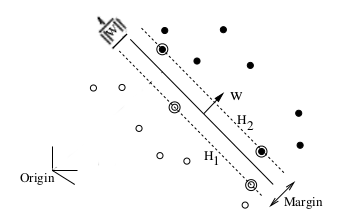
\includegraphics[ width=0.7\textwidth]{Margine}
	\caption[Esempio iperpiano separatore]{Iperpiano separatore per dati linearmente separabili. $H_{1}$ e $H_{2}$ sono paralleli dato che hanno la stessa normale $w$ come si apprezza nelle equazioni \ref{eqn:h1} e \ref{eqn:h2}}
   \label{fig:lsdmar}
\end{figure}

Lo scopo di una \ac{SVM} è:
\begin{enumerate}
\item \label{ite:obj}classificare correttamente il \textit{training set}
\item e selezionare tra quelli che rispettano il punto \ref{ite:obj} quello che generalizza meglio.
\end{enumerate}

Detto succintamente il goal di una \ac{SVM} è trovare l'iperpiano canonico ottimo che separa il \textit{training set} , dove per ottimo si intende quello che massimizza il margine.\\

\subsubsection{Legame con SRM}
\label{subsub:lsrm}
In questa sottosezione si vedrà come la tecnica \textbf{hard margin} di \ac{SVM} è in stretta relazione con \ac{SRM} introdotto nella sottosezione \ref{sub:srm}. Si ha infatti che essendo i dati linearmente separabili la rispondenza con il training set è totale quindi $R_{emp}=0$. Quindi il rischio atteso dipende unicamente dalla \ac{VC} \textit{confidence} che a sua volta dipende dalla \ac{VC} \textit{dimension} $h$. Quindi il classificatore migliore nel caso di \ac{SVM} sarà quello con \ac{VC} \textit{dimension} $h$ minima.  La \ac{SRM} in questo caso diventa una ricerca del classificatore con \ac{VC} \textit{dimension} minima. Si consideri inoltre il seguente teorema:
\begin{teorema}
\label{teo:suphdim}
Sia X un insieme di punti x di uno spazio n-dimensionale  che contiene tutti gli esempi di apprendimento. Sia R il diametro della più piccola ``palla'' (da pensare n-dimesionale) centrata nell'origine che contiene tutti i punti di X. Allora la \ac{VC} dimension ,h, dell'insieme di iperpiani $w \bullet x + b = 0$ aventi margine $\gamma$ è limitata superiormente da: 
\begin{equation*}
h \leq min \biggl( \ceil*{\frac{R^{2}}{\gamma^{2}}} \:\:,\:\: n \biggl) + 1
\end{equation*}
\end{teorema}
Siccome il margine è $\gamma = 2/\norma{w}$ la \ac{VC} \textit{dimension} h più piccola (che abbiamo detto minimizza la \ac{VC} \textit{confidence} e avendo il $R_{emp}$ nullo minimizza anche il rischio atteso) si ottiene per la $\norma{w}$ minima cioè per il margine (pari a $2/\norma{w}$) massimo.  Da quanto detto segue che le \ac{SVM} ricercano l'iperpiano col margine massimo per ottenere il classificatore migliore che da cioè più garanzie di generalizzazione secondo il risultato dell'equazione \eqref{eqn:vapnik} e della \ac{SRM}.
Il discorso è analogo ,ma leggermente differente, nel caso in cui i dati non sono linearmente separabili come nel \textbf{soft-margin}(sottosezione \ref{sub:softmargin}): in questo caso l'errore empirico non è nullo e le \ac{SVM}  nell'ottica di minimizzare il \textit{risk boud} cercano per il migliore compromesso tra gli errori nel \textit{training set} e la massimizzazione del margine .

\subsubsection{Formulazione matematica}
Dalla sottosezione \ref{subsub:lsrm} si evince che \ac{SVM} deve risolvere un problema di programmazione lineare infatti il goal è massimizzare il margine  soggetto a dei vincoli lineari cioè un problema di massimizzazione con vincoli. Ricapitolando dato il \textit{training set} $X$ è necessario trovare tra tutti gli iperpiani che separano i dati (i quali si assume siano linearmente separabili) quello che massimizza il margine, che è pari a $\frac{2}{\norma{w}}$.  Matematicamente si ha:
\begin{alignat*}{2}
&massimizzare \quad&&\frac{2}{\norma{w}} \\
&soggetto \:\:a &&y_i(w \bullet x_i +b) - 1 \geq 0 \qquad \forall i
\end{alignat*} 

Osservando che $\norma{w}^{2} = w \bullet w$ si può dare una formulazione  alternativa ma equivalente che cambia leggermente la natura del problema rendendolo quadratico ma è più conveniente come si vedrà più avanti:
\begin{alignat}{2}
\label{eq:svmpro1}
&minimizzare \quad&&\frac{1}{2}(w \bullet w) \\
\label{eq:svmpro2}
&soggetto \:\:a &&y_i(w \bullet x_i +b) - 1 \geq 0 \qquad \forall i
\end{alignat}
 Per risolvere un problema di \textbf{minimizzazione vincolato} si usano i \textbf{moltiplicatori di Lagrange}. Ad esempio si ha da $\underset{x,y}{minimizzare} \:\: f(x,y)$ col vincolo $g(x,y) = 0$ . Si ha inoltre che $g(x,y) = y+x-1$ allora si ha che $y = 1 - x$ costituisce il cosiddetto \textbf{feasible set} cioè il luogo dei punti dove la soluzione può venire a trovarsi. Lagrange ha dimostrato che la soluzione si ha laddove il gradiente\footnote{Il gradiente è una quantità vettoriale, cioè un vettore espresso tramite le sue componenti. Per i nostri scopi le singole componenti sono formate facendo le derivate parziali della funzione rispetto a ogni singola variabile}  di $f(x,y)$  e quello di $g(x,y)$ puntano nella stessa direzione cioè 
 \begin{equation}
 \label{eq:lag}
 \nabla f(x,y) = \lambda \,\nabla g(x,y)
 \end{equation}
  La quantità scalare $\lambda$ si chiama \textbf{moltiplicatore di Lagrange} e si rende necessaria per il fatto che $\nabla f(x,y) \text{ e } \nabla g(x,y)$ devono avere la stessa direzione ma non necessariamente lo stesso modulo, $\lambda$ è quindi un fattore moltiplicativo che ne tiene conto in modo da eguagliare anche i moduli. Il metodo dei moltiplicatori di Lagrange è valido solo per vincoli di uguaglianza ($g(x,y) = 0$) e in questo caso nelle condizioni per la risoluzione non ci sarà alcun vincolo su $\lambda$. Si definisce la funzione di Lagrange:
 \begin{equation*}
 L(x,y,\lambda) = f(x,y) - \lambda g(x,y) 
 \end{equation*}
 allora 
 \begin{equation*}
 \nabla L(x,y,\lambda) = \nabla f(x,y) - \lambda \, \nabla g(x,y)
 \end{equation*}
e dall'equazione \eqref{eq:lag} si deduce che $\nabla L(x,y,\lambda) = 0$ cioè:
\[
\begin{cases}
\frac{\partial L}{\partial x} = 0 \\
\frac{\partial L}{\partial y} = 0 \\
\frac{\partial L}{\partial \lambda} = 0
\end{cases}
\]
Per trattare casi in cui sono presenti anche dei vincoli di ineguaglianza come nel caso delle \ac{SVM} (vedasi vincoli \eqref{eq:vin}) si utilizzano le \textbf{Karush-Kuhn-Tucker (KKT)} condizioni che consistono nell'imporre --- oltre alle condizioni del metodo dei moltiplicatori di Lagrange per i vincoli di uguaglianza che permangono --- che il moltiplicatore relativo ad ogni vincolo di ineguaglianza venga posto maggiore uguale a 0 , e le condizioni di complementarità che consistono nell'imporre che il prodotto tra un moltiplicatore e il corrispondente vincolo sia uguale a zero. Il metodo dei moltiplicatori di Lagrange  è un caso speciale (sono presenti solo vincoli di uguaglianza) delle KKT condizioni che invece hanno validità generale.
Ad esempio se avessimo due vincoli $g_{1}(x,y) \geq 0 \text{ e } g_{2}(x,y) \geq 0$ si avrebbe che $L(x,y,\lambda_{1},\lambda_{2}) = f(x,y) - \lambda_{1}\,g_{1}(x,y) - \lambda_{2}\,g_{2}(x,y)$ da cui si calcola il gradiente come fatto nell'esempio precedente ottenendo:
\[
\begin{dcases}
\frac{\partial L}{\partial x} = 0 \\
\frac{\partial L}{\partial y} = 0 \\
\frac{\partial L}{\partial \lambda_{1}} = 0 \\
\frac{\partial L}{\partial \lambda_{2}} = 0 \\
\lambda_{1} \geq 0 \\
\lambda_{2} \geq 0
\end{dcases}
\]
I vincoli di complementarità $\lambda_{1}g_{1}(x,y) = 0$ e $\lambda_{2}g_{2}(x,y) = 0$ non sono presenti perchè già posseduti in questo caso.\\
Adesso, alla luce di quanto è stato esposto, si risolverà il problema matematico posto da \ac{SVM} e delineato nelle equazioni \eqref{eq:svmpro1} e \eqref{eq:svmpro2}. Siccome si hanno $l$ vincoli (tanti quanti gli elementi nel \textit{training set}) si deve introdurre un moltiplicatore $\alpha_{i} \text{ con } i=1,\dots,l$ per ognuno degli $l$ vincoli d'ineguaglianza ottenendo il seguente lagrangiano:
\begin{equation}
\label{eq:pri}
L_{p} = \frac{1}{2}\norma{w}^{2} - \sum_{i=1}^{l}\alpha_{i}y_{i}(w \bullet x_{i} + b) + \sum_{i=1}^{l}\alpha_{i}
\end{equation}
dove l'ultima sommatoria scaturisce dal -1 dei vincoli in \eqref{eq:svmpro2}.
Adesso si deve imporre pari a zero $\nabla L_{p}$ ,e siccome è un vettore imporre pari a zero le singole derivate parziali , e imporre le KKT condizioni ottenendo:

\[
\begin{dcases}
\frac{\partial L_{p}}{\partial w} = 0 \\
\frac{\partial L_{p}}{\partial b} = 0 \\
\frac{\partial L_{p}}{\partial \alpha_{i}} = 0 \quad \forall i \\
 \alpha_{i} \geq 0 \quad \forall i \\
\alpha_{i}[y_{i}(w \bullet x_i + b) - 1] = 0 \quad \forall i \\
\end{dcases}
\]
\\\\
che svolgendo le derivate parziali diventa:

\begin{subequations}
\begin{numcases}{}
w - \sum_{i=1}^{l}\alpha_{i}y_{i}x_{i} =0 \label{wvar}\\
\sum_{i=1}^{l}\alpha_{i}y_{i} = 0 \label{bvar}\\
y_{i}(w \bullet x_i + b) - 1 = 0 \quad \forall i \notag \\
 \alpha_{i} \geq 0 \quad \forall i \notag \\
\alpha_{i}[y_{i}(w \bullet x_i + b) - 1] = 0 \quad \forall i \label{vecsup}
\end{numcases}
\end{subequations}

Il problema appena impostato è un problema di programmazione quadratico dato che la funzione obiettivo ($\frac{1}{2}\norma{w}^2$) è quadratica, ma è anche un \textbf{problema convesso di programmazione quadratica} perchè la funzione obiettivo è anche convessa essendo un paraboloide, ed i punti che soddisfano i vincoli cioè il \textit{feasible set} è pure un insieme convesso\footnote{Qualsiasi vincolo lineare definisce un insieme convesso, e un insieme di $N$ vincoli lineari simultanei definisce l'intersezione di $N$ insiemi convessi, che è ancora un insieme convesso.}. Questo sta a significare che si otterrà lo stesso risultato affrontando il problema \textbf{duale} (quello descritto finora è il problema \textbf{primario}) : anzichè minimizzare rispetto alle variabili $w \text{ e } b$ soggetto a vincoli che coinvolgono i moltiplicatori lagrangiani $\alpha$, si massimizza rispetto alle variabili $\alpha$ (variabili duali) soggetto alle relazioni ottenute prima per $w \text{ e } b$ cioè le equazioni \eqref{wvar} e \eqref{bvar} oltre che ad $\alpha_{i} \geq 0$. Alla formulazione duale si possono aggiungere le KKT condizioni della forma primaria che ci forniscono ulteriori informazioni per comprendere la struttura della soluzione. La condizione  \eqref{vecsup} :
\[
\alpha_{i}[y_{i}(w \bullet x_i + b) - 1] \quad \forall i
\]
ci dice che solo i punti del \textit{training set} $x_i$ per i quali $y_{i}(w \bullet x_i + b) = 1$ ,cioè i punti più vicini all'iperpiano separatore (quelli doppiamente cerchiati in figura \ref{fig:lsdmar} sugli iperpiani $H_{1}$ e $H_{2}$ ) , hanno valori $\alpha_{i}$ non nulli. Pertanto solo tali punti contribuiranno al calcolo dei pesi $w$ e per tale motivo sono chiamati \textbf{vettori di supporto}.\\
La formulazione duale del problema è detta \textbf{Wolf duale}, vediamo come si ottiene. Si sostituiscono i vincoli di eguaglianza \eqref{wvar} e \eqref{bvar} riguardanti $b$ e $w$ ($\frac{\partial L_{p}}{\partial w} = 0 \text{ e } \frac{\partial L_{p}}{\partial b} = 0$) nella formulazione primaria cioè nell'equazione \eqref{eq:pri}. Si ha:
\begin{equation}
\begin{split}
&L_{p} = \frac{1}{2}\norma{w}^{2} - \sum_{i=1}^{l}\alpha_{i}y_{i}(w \bullet x_{i} + b) + \sum_{i=1}^{l}\alpha_{i} = \frac{1}{2}(w \bullet w) - \sum_{i=1}^{l}\alpha_{i}y_{i}(w \bullet x_{i} ) \quad\:\: -\\
 &- \sum_{i=1}^{l}\alpha_{i}y_{i}b + \sum_{i=1}^{l}\alpha_{i}
\underset{Si \:sostituisce \:l'equazione \:\eqref{wvar}}{=} \frac{1}{2} \Biggl(\sum_{i=1}^{l}\alpha_{i}y_{i}x_{i} \bullet \sum_{i=1}^{l}\alpha_{i}y_{i}x_{i} \Biggl) \quad\:\:\:\, - \\&
- \Biggl(\sum_{i=1}^{l}\alpha_{i}y_{i}\Bigl(x_{i} \bullet \sum_{j=1}^{l}\alpha_{j}y_{j}x_{j}\Bigl)\Biggl) -\:b\sum_{i=1}^{l}\alpha_{i}y_{i} + \sum_{i=1}^{l}\alpha_{i}
\underset{b \:sparisce\:per \:l'equazione\:\eqref{bvar}}{=} \frac{1}{2} \\&\sum_{i,j = 1}^{l}\alpha_{i}\alpha_{j}y_{i}y_{j}\,(x_{i} \bullet x_{j}) - 
 \sum_{i,j = 1}^{l}\alpha_{i}\alpha_{j}y_{i}y_{j}\,(x_{i} \bullet x_{j}) + \sum_{i=1}^{l}\alpha_{i} \qquad \qquad \qquad \qquad \quad\:\:\,=\\
 &= - \frac{1}{2} \sum_{i,j = 1}^{l}\alpha_{i}\alpha_{j}y_{i}y_{j}\,(x_{i} \bullet x_{j}) + \sum_{i=1}^{l}\alpha_{i}
\end{split}
\end{equation}
quindi si è trovato che la formulazione duale da massimizzare è:
\begin{alignat}{4}
& L_{d} = - \frac{1}{2} \sum_{i,j = 1}^{l}\alpha_{i}\alpha_{j}y_{i}y_{j}\,(x_{i} \bullet x_{j}) + \sum_{i=1}^{l}\alpha_{i} \label{eq:dual}\\
& soggetta \:ai\:vincoli: \nonumber\\
&\sum_{i=1}^{l}\alpha_{i}y_{i} = 0 \quad \forall i \\
&\alpha_{i} \geq 0 \qquad \quad\:\:\: \forall i
\end{alignat}
Si procede come per la forma primale,  cioè imponendo che il lagrangiano della forma duale $L_{d}$ sia pari a zero. Si risolve il sistema, in cui la dipendenza da $w$ e $b$ è sparita (visionare equazione \eqref{eq:dual}), e si trovano gli $\alpha_{i}$.\\
 L'obiettivo finale è trovare l'iperpiano $f(x) = w \bullet x +b$ con i $w \text{ e } b$ cioè la coppia $(w,b)$, che massimizzano il margine. Mediante la formulazione duale si trovano gli $\alpha_i$ che garantiscono i ``migliori'' $(w,b)$ e vengono sostituiti nell'equazione \eqref{wvar} per calcolare il vettore $w$ ricordando che soltanto i \textit{vettori di supporto} ,che hanno $\alpha_{i} \neq 0$, contribuiscono al calcolo di $w$. Quindi si ha: 
\begin{alignat}{3}
f(x)&= w \bullet x +b = \Biggl(\sum_{i=1}^{l}\alpha_{i}y_{i}x_i\Biggl) \bullet x +b = \nonumber\\
&=\Biggl(\sum_{i=1}^{l}\alpha_{i}y_{i}(x_i \bullet x)\Biggl) +b =\nonumber\\
&= \Biggl(\sum_{i \in sv}^{}\alpha_{i}y_{i}(x_i \bullet x)\Biggl) +b \label{eq:test}
\end{alignat} 
Per calcolare $b$ si sostituisce in \ref{eq:test} un elemento $x$ del \textit{training set} --- ed anche la corrispondente etichetta $y$ --- che rappresenta un vettore di supporto, ed i valori ottenuti vengono poi mediati quindi:
\begin{equation}
\label{eq:bhard}
b = \frac{1}{\abs{sv}} \sum_{i \in sv}^{}\Biggl(y_i - \Bigl(\sum_{j \in sv}^{}\alpha_{j}y_{j}(x_i \bullet x_j)\Bigl)\Biggl)
\end{equation}

\subsubsection{Fase di Test}
\label{sub:fte}
Una volta trovati $w$ e $b$, e quindi una volta che la \ac{SVM} è stata \textit{trained} come si usa il classificatore trovato? Immaginiamo di avere un campione n-dimensionale del \textit{test set} $m$ allora si usa l'iperpiano $w \bullet x +b$ per classificare il campione \emph{unseen} $m$ in base all'esito di $sign(w \bullet m + b)$ (l'etichetta di m è 1 oppure -1 in base a $sign(w \bullet m + b)$)

\subsection{Soft Margin}
\label{sub:softmargin}
L'esposizione della sottosezione \ref{sub:cmm} è valida per un \textit{training set} linearmente separabile. Nella maggiore parte dei casi reali i dati tipicamente non sono linearmente separabili cioè non ci sarà una \textit{``feasible region''} perchè non esisterà nessun valore $(w,b)$ ,cioè nessun iperpiano , per cui i vincoli \ref{eqn:h1} e \ref{eqn:h2} siano rispettati. L'idea ,in \cite{Cortes95},è di rilassare tali vincoli  mediante l'introduzione delle \textit{\textbf{variabili slack}} così definite:
\begin{definizione*}
Detta $f$ la funzione caratteristica di un classificatore, che ha come dominio il training set $X$, e un campione $\in X (x_i , y_i)$, si definisce variabile slack del campione, rispetto alla funzione $f$ e al margine $\gamma$, la quantità :
\begin{equation*}
\xi((x_i , y_i) , f , \gamma  ) = \xi_{i} = max(0 , \gamma - y_if(x_i))
\end{equation*}
\end{definizione*}
e il \textit{vettore slack} di $X$ come:
\[ 
\xi = \Braket{\xi_1,\xi_2,\dots,\xi_l}
\] 
Si noti che $\xi_i > \gamma$ indica un'errata classificazione del campione $x_i$.
Quindi i vincoli \ref{eqn:h1} e \ref{eqn:h2} sul \textit{training set} vengono riformulati definendo:
\begin{align}
&w \bullet x_i + b \geq \:\:\:1-\xi_i \qquad \qquad\text{ per } y_i = +1 \label{eqn:h1sm}\\
&w \bullet x_i + b \leq -1+\xi_i \qquad \qquad\text{ per } y_i = -1  \label{eqn:h2sm}\\
&\xi_i \geq 0 \quad \qquad \qquad \qquad \qquad \quad\:\: \forall i \label{eqn:slack}
\end{align}
Un errore in \eqref{eqn:h1sm} e \eqref{eqn:h2sm} occorre quando il corrispondente $\xi_i$ eccede l'unità, ne consegue che $\sum_{i=1}^{l}\xi_i$ è un limite superiore al numero di errori sul \textit{training set}. Allora la funzione obiettivo da minimizzare diventa:
\begin{equation}
\label{eq:softorig}
\frac{1}{2}\norma{w}^2 + Cf\Bigl(\sum_{i=1}^{l}\xi_i^k\Bigl)
\end{equation}
soggetta ai vincoli \eqref{eqn:h1sm} \eqref{eqn:h2sm} e \eqref{eqn:slack}. Il problema appena formulato è convesso  per qualunque $k$ ma si sceglie sempre $k=1$ perchè assicura l'unicità della soluzione (con $k=1$ ne le $\xi_i$ ne i moltiplicatori di Lagrange del problema primale appaiono nel Wolf duale problema come sarà accennato). La soluzione di questo problema di ottimizzazione è chiamato iperpiano \textbf{soft margin}. Inoltre la scelta maggiormente adottata è di approssimare\footnote{Si definisce la norma-1 di un vettore x a l componenti come $\norma{x}_1 = \sum_{i=1}^{l}\abs{x_i}$} $f\Bigl(\sum_{i=1}^{l}\xi_i\Bigl) \text{ con } \Bigl(\sum_{i=1}^{l}\xi_i\Bigl) = \norma{\xi}_1$ per questo talvolta si parla d'iperpiano soft margin norma-1.\footnote{Esiste anche la formulazione norma-2 ma non ci interessa approfondirla}. Il problema originale delineato in \eqref{eq:softorig}  minimizza il numero di errori di classificazione sull'insieme di addestramento ,e quindi minimizza il rischio empirico, ma è un problema NP-completo. Invece con l'approssimazione fatta si minimizza la norma di $\xi$  che non equivale più a minimizzare il numero di errori sui campioni del \textit{training set} ma consiste nel minimizzare gli scostamenti dei punti misclassificati dal nostro iperpiano  mentre determina l'iperpiano con margine massimo  per i restanti punti di $X$. E questo non è più un problema NP-completo. Ricapitolando la formulazione del problema di minimizzazione soft margin\footnote{Si intende da ora in avanti sempre norma-1} è :


\begin{alignat}{3}
\label{eq:softfor}
&minimizzare \quad&&\frac{1}{2}(w \bullet w) + C\sum_{i=1}^{l}\xi_i \\
\label{eq:softvinc}
&soggetto \:\:a &&y_i(w \bullet x_i + b) \geq \:\:\:1-\xi_i \qquad \qquad \\
&\:&&\xi_i \geq 0 \label{eq:softvin2}
\end{alignat}
La scelta di definire la funzione obiettivo \eqref{eq:softfor} tramite la norma risulta ottima dal punto di vista dell'errore di generalizzazione perchè si può dimostrare che quest ultimo è limitato superiormente da una quantità direttamente proporzionale alla norma dello \textit{slack vector} $\xi$, per cui minimizzare la norma consente di minimizzare anche l'errore di generalizzazione.

\subsubsection{Formulazione matematica}
Si  procede alla stessa maniera di hard margin ,cioè per dati linearmente separabili, su dati non linearmenti separabili con la differenza che la funzione obiettivo e anche i vincoli sono cambiati ( equazioni \eqref{eq:softfor} \eqref{eq:softvinc} \eqref{eq:softvin2} ) per tollerare degli errori di classificazione del \textit{training set} e al contempo cercare di massimizzare il margine. Il problema primale diventa:
\begin{equation}
L_p = \frac{1}{2}\norma{w}^2 + C\sum_{i=1}^{l}\xi_i - \sum_{i=1}^{l}\alpha_{i}\{y_i(x_i \bullet w + b) - 1 + \xi_i\} - \sum_{i=1}^{l}\mu_i\xi_i
\end{equation}
Imponendo $\nabla L_p = 0$ e le KKT condizioni si ha:

\begin{subequations}
\begin{numcases}{}
\frac{\partial L_p}{\partial w} = \ w - \sum_{i=1}^{l}\alpha_{i}y_{i}x_{i} =0 \label{wdualsoft}\\
\frac{\partial L_p}{\partial b} = \sum_{i=1}^{l}\alpha_{i}y_{i} = 0 \notag\\
\frac{\partial L_p}{\partial \alpha_i} = y_{i}(w \bullet x_i + b) - 1 + \xi_i = 0 \quad \forall i \notag\\
\frac{\partial L_p}{\partial \xi_i} = C - \alpha_i - \mu_i = 0 \quad \forall i \notag\\
\xi_i \geq 0 \quad \forall i \notag\\
\alpha_i \geq 0 \quad \forall i \notag\\
\mu_i \geq 0 \quad \forall i \notag\\
 \mu_i\xi_i = 0 \quad \forall i \notag\\
 \alpha_i\{y_{i}(w \bullet x_i + b) - 1 + \xi_i\} = 0 \quad \forall i  \notag
\end{numcases}
\end{subequations}

Con dei calcoli analoghi a quanto fatto per il caso linearmente separabile si perviene alla forma duale che consiste nel:
\begin{alignat}{3}
\label{eq:softford}
&massimizzare \quad&&L_{d} = - \frac{1}{2} \sum_{i,j = 1}^{l}\alpha_{i}\alpha_{j}y_{i}y_{j}\,(x_{i} \bullet x_{j}) + \sum_{i=1}^{l}\alpha_{i} \\
\label{eq:softvincd}
&soggetto \:\:a &&0 \leq \alpha_i \leq C \qquad \qquad \\
\label{eq:softvind2}
&\:&&\sum_{i=1}^{l} \alpha_i y_i = 0 
\end{alignat}
Come per hard margin imponendo $\nabla L_d = 0$ e risolvendo si trovano gli $\alpha_i$ che sono usati in \ref{wdualsoft} per calcolare il vettore dei pesi $w$, cui come prima contribuiranno solo i vettori di supporto in quanto sono i soli per cui $\alpha_i \neq 0$:
\begin{equation}
\label{eq:softw}
w = \sum_{i \in sv}^{}\alpha_iy_ix_i
\end{equation}
Il valore di b può essere ricavato come in \eqref{eq:bhard}.
Si osservi come la formulazione duale soft margin sia uguale , fatta eccezione per il vincolo sugli $\alpha_i$ , alla formulazione duale del problema del margine massimo. 

\subsubsection{Parametro C e legami con SRM}
\label{subsub:srmsoft}
Nella funzione obiettivo della formulazione soft margin \eqref{eq:softfor} compare il parametro $C$, talvota detto parametro \textbf{trade-off} , che è essenzialmente un parametro di \textbf{regolarizzazione} che regola il compromesso tra raggiungere un basso errore sul \textit{training set} e minimizzare $\norma{w}$ (cioè massimizzare il margine, che è $2/\norma{w}$ ed avere presumibilmente un minore errore di generalizzazione). Infatti nella forma duale l'unica dipendenza da C è negli $\alpha_i$ nell'equazione \eqref{eq:softvincd} ed avere un valore di $C$ piccolo limita il valore degli $\alpha_i$ e a sua volta del vettore $w$ che come si vede dall'equazione \eqref{eq:softw} aumenta all'aumentare degli $\alpha_i$. Quindi quando $C$ è più piccolo $w$ è pure più piccolo , e quindi il margine è più grande e di conseguenza per il teorema \ref{teo:suphdim} si avranno migliori performances di generalizzazione tuttavia un $C$ piccolo  comporta una minore \textit{accuracy} sul \textit{training set}. Viceversa , per gli stessi motivi, un valore di $C$ più grande classifica meglio il \textit{training set} ma avrà presumibilmente un maggiore errore di generalizzazione. Quindi la regolazione del parametro $C$ è uno step vitale perchè \ac{SRM} è parzialmente implementato tramite la regolazione di questo parametro dato che l'incremento di $C$ incrementa la complessità della classe delle ipotesi ,perchè in ultima analisi aumentare $C$ comporta l'aumento della \ac{VC} \textit{dimension} $h$. Molto spesso per trovare il migliore valore per $C$ si usa la validazione incrociata su vari valori del parametro. Quindi l'implementazione di \ac{SRM} nel soft margin è approssimata tramite la regolazione del parametro $C$.

\subsection{Kernels}
\label{sub:kernels}
L'approccio soft margin per addestrare dati non linearmente separabili non garantisce usualmente ottime prestazioni. Un'alternativa molto potente è quella introdotta in \cite{Vapnik92}. L'idea per gestire dati non linearmente separabili è quella di mappare questi dati in uno spazio di maggiore dimensionalità $\mathcal{H}$ detto \textbf{spazio delle features} o \textbf{spazio delle caratteristiche} in cui i dati diventano lineramente separabili e poi applicare la tecnica hard margin. Questo mapping può essere fatto tramite una funzione $\phi$ siffatta:
\begin{equation*}
\phi : \mathbb{R}^n \to \mathcal{H}
\end{equation*}
L'immagine \ref{fig:kls} illustra quanto appena detto. 

\begin{figure}[htp]
	\centering
	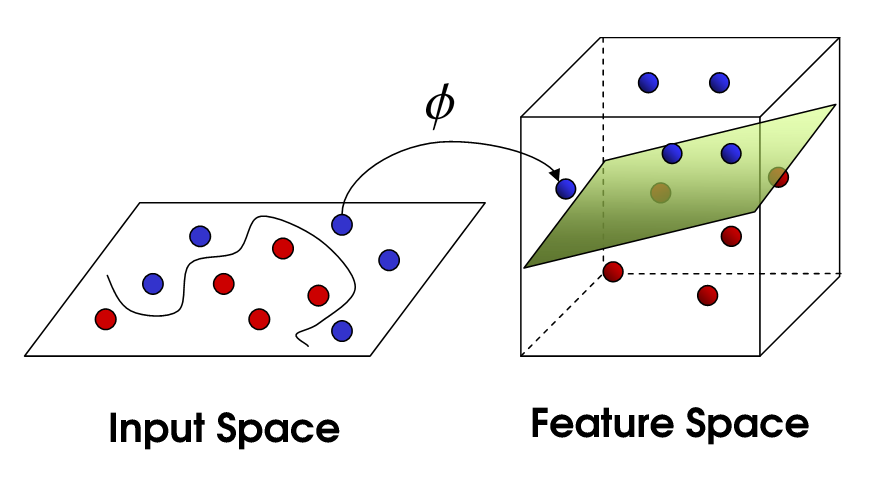
\includegraphics[ width=0.5\textwidth]{KernelLinSepara}
	\caption[Mapping in feature space]{\textit{Dati in $\mathbb{R}^{2}$ resi linearmente separabili ,dalla funzione $\phi$, nello spazio di Hilbert di dimensione tre}}
   \label{fig:kls}
\end{figure}

Inoltre $(x_i \bullet x_j)$ nella formulazione duale in \eqref{eq:dual} diventa $(\phi(x_i) \bullet \phi(x_j))$. Tuttavia utilizzando il \textbf{kernel trick} è possibile pensare di usare una \textbf{kernel function k} tale che
\begin{equation}
\label{eq:kerdef}
k(x_i , x_j) = \phi(x_i) \bullet \phi(x_j)
\end{equation}
che consente di usare il \textit{kernel} K nelle \ac{SVM} senza esplicitamente conoscere $\phi$.
\label{sub:kerc}
Una puntualizzazione su $\phi$ è doverosa. Se $\mathcal{H}$ è di dimensione $M$ $\phi$ può essere una funzione che per calcolare ciascuna delle $M$ coordinate del generico campione $x \in \mathbb{R}^{d}$ nello spazio $H$ utilizza $M$ differenti funzioni cioè:
\[
\phi(x) =[\phi_1(x),\dots,\phi_M(x)]
\]
e allora il kernel diventa:
\begin{equation}
k(x_i , x_j) = \phi(x_i) \bullet \phi(x_j) = \sum_{d=1}^{M}\phi_d(x_i)\phi_d(x_j)
\end{equation}
 Un esempio è il kernel gaussiano nella tabella \ref{tab:kerrem} in cui si dimostra che $\mathcal{H}$ è di dimensione infinita così sarebbe complicato lavorare con $\phi$ esplicitamente. Usando il \textit{kernel trick} si aggira il problema, infatti non vanno più svolti nè il prodotto scalare nè le due valutazioni della funzione $\phi()$ per ogni coppia $(x_i , x_j)$  ma solo la più semplice ed efficiente valutazione del kernel, il quale se rispetta delle determinate condizioni assicura che implicitamente si sta svolgendo un prodotto scalare(ma senza svolgerne il calcolo esplicito che con alte o infinite dimensionalità di $\mathcal{H}$ ,come per il kernel gaussiano in tabella \ref{tab:kerrem} , è impossibile). Un altro esempio chiarificatore in cui i campioni $x$ del \textit{training set} appartengono allo spazio $\mathbb{R}^2$ è il seguente. Dato il \textit{kernel}:
 \begin{equation*}
 k(x_i,x_j) = (x_i \bullet x_j)^2
 \end{equation*}
 è facile trovare una funzione $\phi : \mathbb{R}^2 \to \mathcal{H}$ tale che si ha:
\begin{equation*}
 K(x,y) = (x \bullet y)^2 = \phi(x) \bullet \phi(y) \qquad \text{ con } x,y \in \mathbb{R}^2
\end{equation*}
Infatti se $x=\braket{x_1 , x_2} \text{ e } y=\braket{y_1 , y_2}$ si ha che
\begin{equation}
\label{eq:kernelex}
(x \bullet y)^2 = (x_1y_1 + x_2y_2)^2 = x_{1}^{2}y_{1}^{2} + x_{2}^{2}y_{2}^{2} + 2x_{1}y_{1}x_{2}y_{2}
\end{equation}
e scegliendo $\mathcal{H} = \mathbb{R}^3$ si può avere
 \begin{align*}
    \phi(x) &= \begin{pmatrix}
           x_{1}^2 \\
           \sqrt{2}\,x_{1}x_{2} \\
           x_{2}^2
         \end{pmatrix}
  \end{align*}
 
  quindi:
 \begin{align*}
    \phi(x) \bullet \phi(y) &= \begin{pmatrix}
           x_{1}^2 \\
           \sqrt{2}\,x_{1}x_{2} \\
           x_{2}^2
         \end{pmatrix}\bullet
         \begin{pmatrix}
           y_{1}^2 \\
           \sqrt{2}\,y_{1}y_{2} \\
           y_{2}^2
         \end{pmatrix} = x_{1}^{2}y_{1}^{2} + x_{2}^{2}y_{2}^{2} + 2x_{1}y_{1}x_{2}y_{2}
  \end{align*}

che coincide con quanto ottenuto in \eqref{eq:kernelex}. Inoltre fissato un \textit{kernel} non sono univoci nè i mapping $\phi$ nè la dimensionalità dello spazio $\mathcal{H}$. Per esempio per il \textit{kernel} precedente si sarebbe potuto scegliere $\mathcal{H} = \mathbb{R}^3$ e 
 \begin{align*}
    \phi(x) &= \frac{1}{\sqrt{2}}\begin{pmatrix}
           (x_{1}^2 - x_{2}^2)\\
           2x_{1}x_{2} \\
           (x_{1}^2 + x_{2}^2)
         \end{pmatrix}
  \end{align*}
  oppure $\mathcal{H} = \mathbb{R}^4$ e
  \begin{align*}
    \phi(x) &= \begin{pmatrix}
           x_{1}^2\\
           x_{1}x_{2} \\
           x_{1}x_{2} \\
           x_{2}^2
         \end{pmatrix}
  \end{align*}
Per quanto riguarda $\mathcal{H}$ questo è uno spazio di Hilbert che generalizza lo spazio euclidiano classico, e ha intrinsecamente un \textit{inner product} definito. Comunque non ci si soffermerà su di esso piuttosto è importante comprendere in quali circostanze dato un \textit{kernel} esiste una coppia $(\mathcal{H} , \phi)$ con la proprietà \eqref{eq:kerdef}.
\begin{teorema}[Teorema di Mercer]Dato un kernel continuo e simmetrico\footnote{Simmetrico significa che k(x,y) = k(y,x).} nell'intervallo chiuso    $\overrightarrow{a} \leq \overrightarrow{x} \leq \overrightarrow{b}$ e $\overrightarrow{a} \leq \overrightarrow{y} \leq \overrightarrow{b}$. Allora k(x,y) può essere espanso come
\begin{equation}
k(\overrightarrow{x},\overrightarrow{y}) = \sum_{i=1}^{\infty}\lambda_i\,\phi_i(\overrightarrow{x})\phi_i(\overrightarrow{y})
\end{equation}
con $\lambda_i > 0$. Condizione necessaria e sufficiente affinchè tale espansione sia valida e la sua convergenza assoluta e uniforme è:
\begin{equation*}
\int_{\overrightarrow{b}}^{\overrightarrow{a}}\int_{\overrightarrow{b}}^{\overrightarrow{a}} g(\overrightarrow{x})k(\overrightarrow{x},\overrightarrow{y})g(\overrightarrow{y})\,d\overrightarrow{x}\,d\overrightarrow{y} \geq 0
\end{equation*}

\begin{equation*}
\text{per } \forall g(\cdot) \text{ : } \:\:\int_{\overrightarrow{b}}^{\overrightarrow{a}}g^2(\overrightarrow{x})\,d\overrightarrow{x} < \infty
\end{equation*}
\end{teorema}

Quindi una funzione \textit{kernel} che soddisfa le condizioni del teorema di Mercer rappresenta un prodotto scalare in uno spazio delle features ($\mathcal{H}$) generato da una qualche trasformazione non lineare. Si noti che tale spazio delle features $\mathcal{H}$ può essere infinito e il fatto che $\forall i \:\lambda_i > 0$ implica che il kernel K è semidefinito positivo. Si ha che un kernel simmetrico K semidefinito positivo soddisfa le condizioni del Teorema di Mercer quindi condizione necessaria e sufficiente affinchè un Kernel rappresenti un prodotto scalare in qualche spazio di Hilbert $\mathcal{H}$ è che il kernel sia simmetrico semidefinito positivo.\footnote{\label{note:hessiano}Ad essere simmetrica semidefinita positiva è la matrice associata al kernel. I valori della matrice sono calcolati sulle possibili coppie dei vettori del \textit{training set} cioè su $K(x_i,x_j) \text{ con } i,j=1,\dots,l$ e quindi possono essere raccolti in una matrice $K \in \mathbb{R}^l \times \mathbb{R}^l$ denominata matrice del kernel. E' questa matrice che deve essere simmetrica semidefinita positiva affinchè siano rispettate le condizioni del teorema di Mercer} 

\begin{table}[htp]
\centering
\[ 
\begin{array}{lc} 
\toprule
\text{\textbf{Tipo di Kernel}} & \text{\textbf{k(x , y)}}  \\
\midrule  
\text{Polinomiale}  &  (x \bullet y +1)^p \\
\text{Gaussiano}  &  e^{-\frac{\norma{x-y}^{2}}{2\sigma^2}}\\[1ex]
\text{Iperbolico}  & \tanh(\text{{\footnotesize {\textsl k}}}x \bullet y - \delta) \\

\bottomrule
\end{array}
\]
 \caption[Kernels più noti]{Tipi di kernels più conosciuti}
\label{tab:kerrem}
\end{table}  

Nella tabella \ref{tab:kerrem} si annoverano i kernel predefiniti più noti e maggiormente adottati. Un kernel di per sè non ci dice niente su $\phi$ e la dimensione di $\mathcal{H}$(spazio delle caratteristiche). Tuttavia è stato dimostrato che il \textit{kernel} polinomiale ha per  $\mathcal{H}$ una dimensione di $\binom{n+p-1}{p}$ dove si ricorda che $n$ è la dimensionalità di ogni campione del \textit{training set}. Invece il \textit{kernel} gaussiano ha una dimensionalità di $\mathcal{H}$ infinita. Il suo funzionamento è molto simile alle classiche \textit{Radial Basis Function} infatti  il numero di centri ($\abs{sv}$), i centri stessi (cioè i vettori di supporto) ed i pesi (gli $\alpha_i$) sono prodotti automaticamente da \ac{SVM}. La quantità $\norma{x-y}$ rappresenta la distanza euclidea quadrata e quindi una misura di similarità e il parametro $\gamma = 1/2\sigma^2$ decide il peso di $y$ (se questo è un vettore di supporto) nell'influenzare la classificazione di $x$. Un $\gamma$ piccolo significa un gaussiano con una grande varianza e quindi $y$ (si sottintende che $y$ è un vettore di supporto) avrà un'influenza rilevante su $x$ anche se la distanza tra $x$ e $y$ è grande, al contrario se $\gamma$ è grande la varianza del gaussiano è piccola e $y$ non avrà una influenza molto significativa su $x$ (specie se molto distanti). Le prestazioni del \textit{gaussiano} danno risultati eccellenti paragonabili alle classiche RBF.  Il \textit{kernel} iperbolico è detto anche neurale perchè ricalca da vicino una rete neurale ed in particolare un'unità sigmoidale a due strati. Il primo strato consiste in $\abs{sv}$ insiemi di pesi, ed ogni insieme consta $n_l$ (la dimensionalità dei campioni) pesi, e il secondo strato consiste di $\abs{sv}$ pesi (gli $\alpha_i$) cosicché una valutazione richiede di prendere una somma pesata dei sigmoidi, essi stessi valutati sul prodotto scalare dei dati nel \textit{test set} con i vettori di supporto. Il \textit{kernel} iperbolico-neurale è poco utilizzato perchè solo per alcuni specifici valori di {\footnotesize {\textsl k}} ,$\delta$ e dei dati $x$ le condizioni del teorema di Mercer sono soddisfatte ed è stato dimostrato che molte combinazioni dei parametri ci si riconduce al \textit{kernel} gaussiano.\\
La ragione per mappare i campioni dallo spazio originario in uno spazio a dimensione molto superiore (\textit{feature space} che come visto per il \textit{kernel} gaussiano può essere anche infinita) è il \textbf{teorema di Cover sulla separabilità} \cite{Cover65}:
\begin{teorema}
\label{teo:Cover}
Un problema di classificazione complesso, formulato attraverso una classificazione non lineare dei dati ad altà dimensionalità, ha maggiore probabilità di essere linearmente separabile che in uno spazio a bassa dimensionalità.
\end{teorema}

\subsubsection{Formulazione matematica}
Come indicato dal teorema \ref{teo:Cover} nello spazio $\mathcal{H}$ si avrà presumibilmente una lineare separazione dei dati e questo consente di utilizzare la formulazione hard margin in \eqref{eq:dual}  che resta pressochè invariata. L'unica sostituzione da fare è nell'utilizzo del mapping nel prodotto scalare. Quindi la nuova formulazione  con kernel diventa:

\begin{alignat}{4}
& L_{d} = - \frac{1}{2} \sum_{i,j = 1}^{l}\alpha_{i}\alpha_{j}y_{i}y_{j}\,(\phi(x_{i}) \bullet \phi(x_{j})) + \sum_{i=1}^{l}\alpha_{i} = - \frac{1}{2} \sum_{i,j = 1}^{l}\alpha_{i}\alpha_{j}y_{i}y_{j}\,k(x_{i} ,  x_{j}) + \sum_{i=1}^{l}\alpha_{i} \label{eq:Kerdual}\\
& soggetta \:ai\:vincoli: \nonumber\\
&\sum_{i=1}^{l}\alpha_{i}y_{i} = 0 \quad \forall i \nonumber\\
&\alpha_{i} \geq 0 \qquad \quad\:\:\: \forall i \nonumber
\end{alignat}

Anche in fase di test non ci sono problemi dato che  la classificazione del campione di test $x$ scaturisce dalla valutazione di $sign(w \bullet \phi(x) +b)$ ma $w = \sum_{i =1}^{\abs{sv}}y_i\alpha_i\phi(x_i)$ dove gli $x_i$ sono i vettori di supporto. Quindi sostituendo si ha:
\begin{equation}
sign\Bigl(\sum_{i=1}^{\abs{sv}}\alpha_iy_i\phi(x_i) \bullet \phi(x) + b \Bigl)= sign\Bigl(\sum_{i=1}^{\abs{sv}}\alpha_iy_i\,k(x_i , x) + b\Bigl)
\end{equation}
quindi anche in fase di test non abbiamo la necessità di calcolare $\phi$ che comporterebbe l'effettuazione di prodotti scalari di vettori con un numero di componenti eleveto se non addirittura infinito (come il \textit{kernel} gaussiano). E' proprio questo il vantaggio che apporta il \textbf{kernel trick}.

\subsubsection{Prodotto scalare come misura di similarità}
\label{subsub:prscal}
Il motivo per cui si predilige la formulazione duale rispetto a quella primaria è da ricercare nel fatto che in essa compare il prodotto scalare che come visto conduce alla tecnica dei \textit{kernels}. Un altro motivo è che il prodotto scalare è una \textbf{misura di similarità} e quindi trascendendo i \textit{kernels} classici della tabella \ref{tab:kerrem} ,se si rivelano inappropriati, è possibile definire un \textit{kernel} su misura che implicitamente definisce una misura di similarità \textit{customizzata} tra i campioni. Riferendoci ,senza perdere di generalità,alla formulazione duale hard margin in \eqref{eq:dual} \footnote{Per la formulazione con kernels la misurà di similarità è relativa ai campioni trasformati cioè a $\phi(x_i) \bullet \phi(x_j)$} si cerca di interpretare più in dettaglio come funziona il prodotto scalare ricordando che $L_d$ va massimizzato. Assumendo che $x_i$ e $x_j$ sono due campioni  si ha che:
\begin{enumerate}
\item Se $x_i \text{ e } x_j$ sono \textbf{completamente dissimili} come in figura \ref{fig:dissp} il prodotto scalare è zero e non contribuiscono a $L_d$ (anche se non sono esattamente ortogonali ma quasi il prodotto scalare sarà piccolo ed anche il contributo a $L_d$).
\item Se $x_i \text{ e } x_j$ sono \textbf{completamente simili} (o quasi) cioè il loro prodotto scalare è uno (o quasi uno) si può fare un ulteriore distinguo:
\begin{itemize}
\item $y_i \text{ e } y_j$ cioè le rispettive etichette sono uguali (cioè entrambe 1 o entrambe -1), allora siccome $\alpha_i,\alpha_j \geq 0$ $\alpha_i\alpha_jy_iy_j(x_i \bullet x_j)$ per quei due specifici campioni $x_i,x_j$ è positivo (o nullo) ma moltiplicato per -1/2 è negativo quindi $L_d$ diminuisce. Se ne deduce che campioni simili (prodotto scalare uguale o vicino a uno) con la stessa etichetta come in figura \ref{fig:simpsamelab} sono ignorati da \ac{SVM} (perchè altrimenti il margine diminuirebbe) e quindi \ac{SVM} non li rende vettori di supporto.
\item $y_i \text{ e } y_j$ cioè le rispettive etichette sono opposte (cioè 1 e -1 o viceversa). Inoltre i vettori sono simili e il prodotto scalare è vicino a 1 come in figura \ref{fig:simpdifflab} quindi $\alpha_i\alpha_jy_iy_j(x_i \bullet x_j) \leq 0$ e moltiplicato per -1/2 diventa positivo e quindi contribuisce ad incrementare il margine. Quindi \ac{SVM} renderà tali elementi del \textit{training set} vettori di supporto (perchè fanno aumentare il margine) 
\end{itemize}
\end{enumerate}

\begin{figure}[htp]
	\centering
	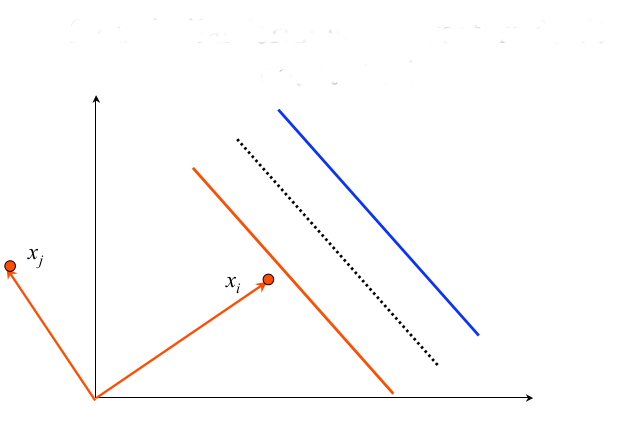
\includegraphics[ width=0.5\textwidth]{VettoriDissimili}
	\caption[Campioni dissimili]{\textit{Due campioni dissimili(ortogonali), indipendentemente dall'etichetta, non contano affatto.}}
   \label{fig:dissp}
\end{figure}

\begin{figure}[htp]
	\centering
	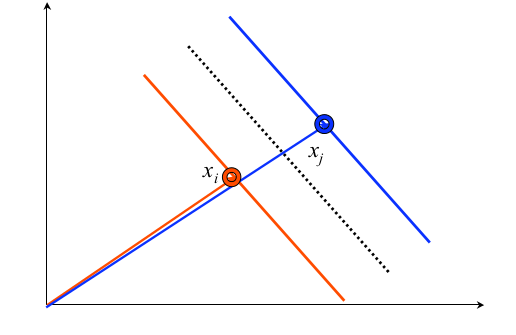
\includegraphics[ width=0.5\textwidth]{VettoriSimiliDifferenteLabel}
	\caption[Campioni simili differenti etichette]{\textit{Due campioni molto simili,$x_i$ e $x_j$, con etichette diverse, tendono a massimizzare il margine e sono resi vettori di supporto.}}
   \label{fig:simpdifflab}
\end{figure}

\begin{figure}[htp]
	\centering
	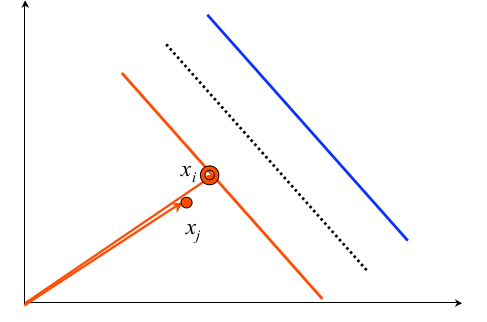
\includegraphics[ width=0.5\textwidth]{VettoriSimiliUgualeLabel}
	\caption[Campioni simili differenti etichette]{\textit{Due campioni molto simili,$x_i$ e $x_j$, con etichette uguali, tendono a minimizzare il margine e quindi non vanno resi vettori di supporto. Oppure se uno di loro è un vettore di supporto (perchè con altri campioni contribuisce ad aumentare il margine) l'altro non va reso un vettore di supporto (in modo da avere coefficiente nullo) in modo da non influenzare negativamente il margine.}}
   \label{fig:simpsamelab}
\end{figure}

\subsubsection{String kernels}
\label{subsub:stk}
Come accennato in precedenza in \ref{subsub:prscal} in determinati ambiti è possibili definire un \textit{kernel} che rappresenta una misura di similarità adatta allo specifico problema da affrontare o in cui gli elementi del \textit{training set} sono strutturati, come ad esempio stringhe ed alberi. Un esempio molto importante , e rilevante ai fini della tesi, è quello dei \textbf{string kernels}, dei quali  è possibile trovare un'introduzione in \cite[p. 60]{DeLaHiguera10}. In questa sede a titolo esemplificativo se ne descriveranno un paio. In generale l'obiettivo di uno \textit{string kernel} è quello di rappresentare o estrapolare delle features delle stringhe che possono essere rilevanti per un problema specifico in termini di similarità o dissimilarità. Uno dei più semplici è il \textbf{Parikh kernel} che associa ad ogni stringa un vettore di numeri naturali dove ogni componente è il numero di occorrenze di un simbolo dell'alfabeto nella stringa. La dimensione del \textit{feature space} dipende dal numero di elementi nell'alfabeto. Si consideri l' esempio nella tabella \ref{tab:parker} in cui si hanno quattro elementi del \textit{training set} $\{bac , baa , cab , bad\}$ e i quattro simboli dell'alfabeto $\{a,b,c,d\}$ che rappresentano le funzioni $\phi_{1}\text{,}\phi_{2}\text{,}\phi_{3}\text{,}\phi_{4}$ che mappano gli elementi nel \textit{feature space}. Si ha allora che la valutazione del \textit{kernel} tra gli elementi $bad \text{ e } baa$ è
\begin{equation*}
k(bad , baa) = 1\cdot2 + 1\cdot1 + 0\cdot0+1\cdot0 = 3
\end{equation*}
Un altro \textit{string kernel} molto noto è \textbf{all k-subsequences kernel} che calcola il prodotto scalare di due vettori in cui ogni componente è il numero di occorrenze di sottosequenze (che si ricorda possono essere contigue o non contigue) di lunghezza al più $k$ in una stringa. Nella tabella \ref{tab:all2subker} vi un esempio di \textit{All 2-subsequences kernel}.\footnote{Dalla tabella nell'esempio per motivi di spazio sono omesse le \textit{features}, cioè le sottosequenze , per le quali tutti i campioni hanno valore zero come ad esempio la sottosequenza $cc$} Si ha allora che la valutazione del \textit{kernel} nell'esempio tra gli elementi $bad \text{ e } baa$ è
\begin{equation*}
k(bad , baa) =  6
\end{equation*} 
\textbf{All k-subsequences kernel} ha sempre almeno valore 1 per la presenza della $feature$ $\lambda$ cioè la stringa vuota che è sottosequenza di ogni stringa. Anche per i \textit{string kernels} tipicamente non si calcolano le funzioni $\phi$ e i relativi prodotti scalari ma si usa il \textit{kernel trick} che viene realizzato tramite tecniche di programmazione dinamica. Per un'implementazione di molti dei più noti \textit{string kernels} compresi quelli esposti in questa sede si veda \cite{Cristianini04}.
I kernel non sono solo un escamotage per renderne efficiente il calcolo, che comunque in alcuni casi come uno spazio delle caratteristiche enorme o infinito sarebbe impossibile, ma hanno due pregi notevoli che rendono \ac{SVM} molto versatile ed applicabile nei più svariati contesti:
\begin{enumerate}
\item Consentono di trattare con elementi del \textit{training set} che non sono in forma vettoriale ma che sono strutturati come ad esempio alberi e grafi
\item Consentono di trattare con elementi del \textit{training set} che hanno lunghezza differente infatti finora si è sottaciuto che le \ac{SVM} nella loro formulazione senza \textit{kernel} possono funzionare solo con elementi della stessa lunghezza. Una trasformazione $\phi$, implicitamente indotta da un kernel che rispetta le condizioni di Mercer, uniforma le stringhe alla stessa lunghezza $M$ (M è la dimensione dello spazio di Hilbert $\mathcal{H}$) e quindi permette di trattare anche campioni di lunghezza diversa.
\end{enumerate}

\begin{table}[htp]
\centering 
\begin{tabular}{lcccc} 
\toprule
\multirow{2}*{Dati} &  $\phi_1$ &  $\phi_2$ &  $\phi_3$ &  $\phi_4$\\
\cmidrule(lr){2-5}
& $a$ & $b$ & $c$ & $d$  \\
 \midrule  
bac  &  1 & 1 & 1 & 0 \\ 
baa  &  2 & 1 & 0 & 0 \\
cab  &  1 & 1 & 1 & 0 \\
bad  &  1 & 1 & 0 & 0 \\
\bottomrule
\end{tabular}
\caption[Parikh kernel]{\textit{Parikh kernel su quattro stringhe e su un alfabeto quaternario}}
\label{tab:parker}
\end{table}    




\begin{table}[htp]
\centering 
\begin{tabular}{lcccccccccccccc} 
\toprule
\multirow{2}*{Dati} &  $\phi_1$ &  $\phi_2$ &  $\phi_3$ &  $\phi_4$ &  $\phi_5$ &  $\phi_6$ &  $\phi_7$ &  $\phi_8$ &  $\phi_9$ &  $\phi_{10}$ &  $\phi_{11}$ &  $\phi_{12}$ &  $\phi_{13}$ &  $\phi_{14}$\\
\cmidrule(lr){2-15}
& $\lambda$ & $a$ & $b$ & $c$ & $d$ & $aa$ & $ab$ & $ac$ & $ad$ & $ba$ & $bc$ & $bd$ & $ca$ & $cb$  \\
 \midrule  
bac  &  1 & 1 & 1 & 1 &  0 & 0 & 0 & 1  &  0 & 1 & 1 & 0 &  0 & 0 \\ 
baa  &  1 & 2 & 1 & 0 &  0 & 1 & 0 & 0  &  0 & 2 & 0 & 0 &  0 & 0 \\
cab  &  1 & 1 & 1 & 1 &  0 & 0 & 1 & 0  &  0 & 0 & 0 & 0 &  1 & 1 \\
bad  &  1 & 1 & 1 & 0 &  1 & 0 & 0 & 0  &  1 & 1 & 0 & 1 &  0 & 0 \\
\bottomrule
\end{tabular}
 \caption[All 2-subsequences kernel]{\textit{All 2-subsequences kernel su quattro stringhe e su un alfabeto quaternario}}
\label{tab:all2subker}
\end{table}

\subsection{Versione soft margin kernelized}
Le tecniche esposte nelle sottosezioni \ref{sub:kernels} e \ref{sub:softmargin} sono combinate insieme per ottenere la versione delle \ac{SVM} di riferimento maggiormente adottata. Infatti sebbene i  \textit{kernels} rendano presumibilmente il \textit{training set} linearmente separabile non c'è alcuna garanzia che questo avvenga realmente. Inoltre anche se i deti vengono resi linearmente separabili è consigliabile utilizzare ugualmente la tecnica soft margin anzichè quella del classificatore a margine massimo (hard margin) perchè può accadere che a causa della presenza di alcuni \textbf{\textit{outliers}}\footnote{Sono delle anomalie cioè degli elementi del \textit{training set}, tipicamente in numero esiguo, che si discostano nettamente dal resto dei campioni} ci sia \textit{overfitting} , cioè eccessivo adattamento al \textit{training set} e scarsa capacità di generalizzare , che potrebbe essere scongiurato scegliendo un \textbf{decision boundary}\footnote{cioè un iperpiano separatore} con soft margin che anche se ignora gli \textit{outliers} misclassificandoli porta alla scelta di un iperpiano separatore con un margine più grande e quindi con migliori capacità di generalizzare. Per questa ragione anche se la scelta di un kernel rendesse i dati lineramente separabili (asserzione che comunque non è sempre verificata) si predilige soft margin ad hard margin per cui usualmente la versione di riferimento di \ac{SVM} combina i \textit{kernels} con soft margin e la formulazione matematica del problema duale da risolvere diventa:
\begin{alignat}{3}
\label{eq:softford2}
&massimizzare \quad&&L_{d} = - \frac{1}{2} \sum_{i,j = 1}^{l}\alpha_{i}\alpha_{j}y_{i}y_{j}\,k(x_{i} , x_{j}) + \sum_{i=1}^{l}\alpha_{i} \\
\label{eq:softvincd2}
&soggetto \:\:a &&0 \leq \alpha_i \leq C \qquad \qquad \\
&\:&&\sum_{i=1}^{l} \alpha_i y_i = 0 
\end{alignat}

\subsection{Globalità e unicità della soluzione}
\label{sub:globuni}
Uno dei vantaggi delle \ac{SVM} rispetto alle reti neurali è che assicurano una soluzione deterministica nel senso che dato un \textit{training set} la soluzione non dipende da elementi aleatori cosa che accade nelle reti neurali dove l'inizializzazione casuale dei pesi può condurre a una soluzione differente da un'esecuzione all'altra. Un altro vantaggio delle \ac{SVM} è che essendo un problema di programmazione quadratica convessa con vincoli lineari assicura di trovare una soluzione globale mentre nelle reti neurali si ha la certezza di trovare un minimo locale ma non è assicurato di trovare la soluzione migliore. Nelle \ac{SVM} il rispetto delle  KKT condizioni è una condizione necessaria per trovare un minimo o un massimo globale ma in generale non sono condizioni sufficienti cioè vi è solo la garanzia di un minimo locale. Tuttavia la natura convessa del problema, rende le condizioni KKT anche sufficienti, assicura che la soluzione trovata sia sempre quella globale e questo è il motivo per cui si usa la formulazione quadratica alternativa in \ref{eq:svmpro1}. Ma è necessario garantire anche l'\textbf{unicità} della soluzione $\{w,b\}$ perchè potrebbero esistere delle altre coppie $\{w,b\}$ che siano pure soluzione (esistenza più minimi globali equivalenti) oppure la stessa soluzione, ma con una diversa espansione di $w=\sum_{i=1}^{\abs{sv}}\alpha_iy_ix_i$ e questo è pure rilevalente perchè potrebbe essere un'espansione migliore con meno vettori di supporto\footnote{Una soluzione con tanti vettori di supporto vicino al numero di elementi nel \textit{training set} è indice di \textit{overfitting}.}.
E' garantito che la soluzione sia unica se la formulazione duale \ref{eq:dual} o la formulazione duale con \textit{kernel} \ref{eq:Kerdual} è strettamente convessa. Anzichè le formulazioni \ref{eq:dual} e \ref{eq:Kerdual} si può definire l'\textbf{Hessiano} del problema che è una formulazione matriciale ottenuta come descritto nella nota \ref{note:hessiano}. Si ha che:
\begin{teorema*} Un problema quadratico è strettamente convesso se e solo se l'Hessiano associato è definito positivo.
\end{teorema*}
Quando l'Hessiano non è definito positivo la natura convessa del problema assicura che l'Hessiano sia comunque  almeno semidefinito positivo cosa che assicura la globalità della soluzione ma non l'unicità.  Riassumendo la globalità della soluzione è sempre garantita. L'unicità è garantita solo se l'Hessiano è definito positivo. 

\subsection{Dati non bilanciati}
\label{sub:unbalanced}
Una situazione che merita un approfondimento è quando i dati del \textit{training set} sono sbilanciati cioè  i dati con un'etichetta positiva superano significativamente i dati con etichetta negativa o viceversa. Il quesito cui si deve rispondere è se un \textit{training set} sbilanciato influenza o meno il funzionamento di \ac{SVM}. Innanzitutto si ricorda che nella formulazione soft margin e anche quella soft margin combinata con l'uso di un \textit{kernel} minimizzare la funzione obiettivo significa minimizzare l'errore sul \textit{training set} (errore empirico) e massimizzare il margine (cioè minimizzare $\norma{w}$) simultaneamente e il parametro C controlla il compromesso tra queste due quantità. Ponendoci, a titolo esemplificativo , nel caso in cui i campioni positivi sono molto meno di quelli negativi si ha che l'iperpiano separatore si muoverà nella direzione opposta a dove sono la maggior parte dei campioni negativi al fine di produrre un margine più grande col prezzo da pagare che è quello di incrementare gli errori di classificazione degli esempi positivi. Ma dato che i campioni positivi sono in minoranza l'errore di classificazione dei campioni positivi non sarà particolarmente significativo e complessivamente il valore della funzione obiettivo sarà minimizzato, che è il goal di \ac{SVM}. Questo comporta un \textit{overfitting} al \textit{training set} che poi avrà delle ripercussioni negative in fase di generalizzazione dato che il classificatore ottenuto si comporterà in maniera simile a un classificatore \textit{majority class}\footnote{E' un classificatore che assegna a tutti i campioni la stessa etichetta(o positiva o negativa)}. Esistono diversi approcci per affrontare questo problema ad esempio quello proposto in \cite{Zhang05}\footnote{La tecnica proposta in questo riferimento è applicata per una formulazione leggermente diversa di \ac{SVM} detta WPSVM tuttavia è valida anche per le \ac{SVM} classiche} in cui si assegna un peso $\sigma_i$ ad ogni variabile slack $\xi_i$.  Si impone un bilanciamento sull'errore accumulativo (su tutte le variabili slack) tra campioni positivi e negativi(cioè si impone che il contributo all'errore globale dei campioni positivi sia uguale al contributo di quelli negativi cioè che: 
\begin{equation*}
\sum_{y_{i}=1}^{}\sigma_{+}^{2}\xi_{i}^2=\sum_{y_{i}=-1}^{}\sigma_{-}^{2}\xi_{i}^2
\end{equation*}
 usando la formulazione soft-margin norma-2) e assumendo che l'errore è uguale su ogni campione si ottiene un valore globale(slegato dal singolo campione) del peso degli errori e si può scrivere $N_{+}\sigma_{+}^{2} =N_{-}\sigma_{-}^{2} $ dove $N_{+} \text{ e } N_{-}$ sono rispettivamente il numero di campioni positivi e di quelli negativi. Imponendo $\sigma_{-}=1$ si ottiene $\sigma_{+}=\sqrt{N_{-}/N_{+}}$ (anche se in realtà si utilizza una formulazione leggermente diversa) in modo da usare un unico parametro(perchè $\sigma_{-}=1$) per trattare con \textit{training set} non bilanciati  anzichè due. Aggiungendo questo parametro e cambiando leggermente la formulazione di \ac{SVM} (splittando la sommatoria per variabili slack positive e negative) si dovrebbe ottenere un classificatore che sulla carta riesce a ottenere risultati migliori a partire da \textit{training set} non bilanciati.
 
 \subsection{Algoritmo di ottimizzazione}
 La rappresentazione matematica del problema che \ac{SVM} intende risolvere --- che nella sua espressione ultima è rappresentata dalla forma duale e dai relativi vincoli ,nelle quattro formulazioni precedentemente esposte  --- si approccia tipicamente con metodi numerici anzichè ricercare una soluzione analitica. In questa sede non interessa descrivere nel dettaglio i vari risolutori esistenti ma soltanto esporne le linee guida in modo da potere comprendere alcuni dei parametri dei \textit{tools software} che implementano \ac{SVM}. \\
 L'approccio alla soluzione di questo tipo di problemi è iterativo: si parte da un punto all'interno della \textit{feasible region} e ci si muove non lasciando tale regione e cercando di massimizzare il valore della funzione obiettivo, fino a che non risulta soddisfatto qualche criterio. I criteri per determinare la convergenza  possono essere ottenuti sfruttando le caratteristiche dei sistemi convessi. Questi sono essenzialmente tre:
 \begin{itemize}
 \item \textbf{Controllare la crescita della funzione duale}\\Tale funzione raggiunge il massimo nella soluzione. Controllare il valore della funzione e, specialmente il suo aumento ad ogni passo, fornisce un semplice criterio di convergenza. L'addestramento si ferma quando il rapporto di crescita scende sotto una certa soglia. Sfortunatamente , questo criterio si è dimostrato non sempre affidabile.
 \item \textbf{Gap di ammissibilità}\\All'ottimo, la differenza tra il valore della funzione obiettivo del problema in forma primale e del problema duale è nulla. Di conseguenza, un possibile criterio è quello di monitorare tale differenza nota come \textit{gap di ammissibilità}.
 \item \textbf{Monitorare il soddisfacimento delle condizioni KKT}\\Esse sono condizioni necessarie e sufficienti (in caso di problemi convessi come quello delle \ac{SVM}) per la convergenza, per cui ne forniscono un criterio naturale.
 Ovviamente questi criteri vanno verificati all'interno di un certo margine di tolleranza.
 \end{itemize}
 Molto importante,in ogni caso, è il livello di tolleranza utilizzato per verificare il criterio di convergenza scelto. Una accuratezza eccessivamente elevata potrebbe comportare un tempo di esecuzione dell'algoritmo altrettanto elevato ed ingiustificato dal punto di vista dei risultati ottenuti.
 
 \section{SVM$^{light}$}
 \label{sec:light}
 Questa tesi è volta a costruire un classificatore che approssimi un \textit{Oracolo} a partire da un insieme di campioni labellati usando come modello le \ac{SVM}. Quindi è stato necessario scegliere una delle tante implementazioni di \ac{SVM} e tra le più note e utilizzate si hanno senz altro \textbf{LIBSVM} e \textbf{SVM$^{light}$}. La scelta è ricaduta su SVM$^{light}$   di Thorsten Joachims perchè è sembrato un tool più semplice da modificare e \textit{customizzare} ed essendo un' implementazione di \ac{SVM} in linguaggio C relativamente semplice da includere all'interno della libreria GI-leraning che è scritta in C++. SVM$^{light}$ è particolarmente adatto per problemi di \textit{text classification} ma essendo un tool generico è adatto a tutti i problemi di classificazione binaria compreso la classificazione di stringhe che interessa in questa sede. Inoltre consente l'utilizzo di un \textit{kernel} personalizzato come uno \textit{string kernel}. Malgrado il porting in GI-leraning, la classificazione binaria,la definizione di un kernel personalizzato fosse possibile anche in LIBSVM la scelta è ricaduta su  SVM$^{light}$ perchè quest'ultima è sembrata più semplice da personalizzare ai propri fini.Il lato negativo della medaglia è stato che a causa dell'assenza nativa  di strumenti predefiniti in SVM$^{light}$ come la \textit{cross validation},lo \textit{scaling}, metodi di ricerca dei parametri come \textit{grid-search} ecc. è stato necessario implementare questi strumenti per fruirne. In questo modo si è però avuto pieno controllo di quello che si stesse facendo senza dovere usare implementazioni di terzi (escluso le \ac{SVM} stesse),in alcuni casi poco documentate, a scatola chiusa. SVM$^{light}$ mette a disposizione il calcolo di accuracy,precision e recall sul \textit{test set} , un calcolo efficiente ma solo approssimativo di Leave-One-Out.
 
SVM$^{light}$ è descritto alla pagina di riferimento: \href{http://svmlight.joachims.org/}{http://svmlight.joachims.org/}. Qui sarà trattato solo il caso della classificazione binaria. SVM$^{light}$ consiste di due eseguibili, svm\_learn per addestrare il \textit{training set} ed \textit{svm\_classify} per fare predizioni sui nuovi dati usando il modello precedentemente  trovato. Tipicamente si avrà un train\_file contenente il \textit{training set} e un test\_file contenente il \textit{test set}. Entrambi i file devono rispettare un ben preciso formato. \\Il primo step è addestrare una \ac{SVM} ad esempio con il seguente comando:
\begin{equation*}
\text{svm\_learn -c 1.5  -x 1  train\_file  model\_file}
\end{equation*}
che scrive il modello trovato alla fine dell'addestramento sul file model\_file. c ed x sono dei parametri che saranno accennati più avanti. In model\_file ci sarà il valore di b dell'iperpiano separatore e una riga per ogni vettore di supporto che inizierà con il corrispondente valore $\alpha_iy_i$. Per fare predizioni sul test set si usa il comando:
\begin{equation*}
\text{svm\_classify test\_file model\_file prediction\_file}
\end{equation*}
Il comando legge il \textit{test set} dal file di testo e l'iperpiano trovato in precedenza da model\_file e scrive la predizione fatta tramite l'iperpiano su prediction\_file. L'ordine delle linee in prediction\_file corrisponde all'ordine in test\_file (ad esempio la prima riga in prediction\_file indica la predizione del primo campione in test\_file). In prediction\_file ci sono dei valori che indicano la distanza dall'iperpiano (dal modello) ed il segno determina la classe predetta.

\subsection{Formato dei file}
Sia train\_file che test\_file hanno il seguente formato:
\begin{equation*}
<y>\:\: <numeroFeature>:<valore> \:\dots\: <numeroFeature>:<valore>
\end{equation*}
<y> indica la classe del campione cioè può essere 1,-1,0. Il valore 1 indica un campione positivo, -1 un campione negativo , 0 un campione del \textit{test set} di cui non si conosce la classe di appartenenza e si vuole che sia \ac{SVM} a predirla. Tuttavia nel caso in cui test\_file contenga per ogni riga, cioè ogni campione, l'etichetta corretta anzichè 0  saranno riportate in output varie misure (accuracy,precision,recall ecc.) che sono misure orientative sulle capacità di generalizzare del predittore trovato (l'iperpiano) (cioè si conoscono le corrette etichette dei campioni nel \textit{test set} e si vuole capire se il modello trovato fa le corrette predizioni per questi campioni). Ogni coppia <numeroFeature>:<valore> indica il valore di una particolare \textit{feature} (cioè componente) di un campione. Per esempio, 3:0.7 5:0.1  specifica il campione $x=(0,0,0.7,0,0.1)$ infatti le features non esplicitamente specificate sono pari a 0 per default. Le coppie devono essere ordinate per numero di feature crescente. Il più piccolo numero di una feature è 1.

\subsection{Parametri}
Saranno introdotti e spiegati solo i parametri utlizzati nel lavoro sperimentale di tesi:\\
\begin{itemize}
\item [\textbf{-v}] Indica il livello di verbosità delle stampe in output. Il valore di default è 1.
\item [\textbf{-x}] Se impostato a 1(default 0) calcola un'approssimazione di LOO.
\item [\textbf{-c}]  E' il parametro \textit{trade-off C} introdotto nella formulazione soft-margin. Il migliore valore di C dipende dai dati e va determinato empiricamente. Assume un valore decimale.
\item [\textbf{-j}] E' il parametro fattore di costo e scaturisce da un ragionamento del tutto analogo a quello fatto in \ref{sub:unbalanced} per tenere conto di dati non bilanciati. Joachims utilizza una formulazione  soft margin (norma-1):\begin{equation*}\frac{1}{2}\norma{w}^2 + C_{+}\sum_{i:y_i=1}\xi_i + C_{-}\sum_{j:y_j=-1}\xi_j\end{equation*} che impostando $j=N_-/N_+$ diventa:
\begin{equation*}
\frac{1}{2}\norma{w}^2 +C\Biggl(j\sum_{i:y_i=1}\xi_i + \sum_{j:y_j=-1}\xi_j\Biggl)
\end{equation*}
j quindi è statico nel senso che non va ricercato con questo escamotage con una validazione incrociata, a differenza di C. Quindi questo parametro funge da peso e se ad esempio i campioni negativi sono il doppio di quelli positivi j=2 ed i campioni positivi saranno pesati con un peso maggiore di quelli negativi.
\item [\textbf{-t}] Seleziona il tipo di kernel:
\begin{itemize}
\item[0:] lineare(default)
\item[1:] polinomiale
\item[2:] gaussiano
\item[3:] sigmoidale
\item[4:] personalizzato

\end{itemize}
\item[\textbf{-g}] E' il parametro $\gamma$ del kernel gaussiano.
\item[\textbf{-e}] E' un parametro di ottimizzazione. Imposta la tolleranza per il criterio di terminazione nell'algoritmo di risoluzione di SVM$^{light}$ tra un'iterazione e l'altra. Di default è 0.001 Aumentare questo valore comporta una fase di addestramento più veloce, ma aumentarlo troppo può condurre a trovare un iperpiano con scarse performances.
\end{itemize}
 
 
 
 
 
 
 
 
 
 \chapter[Prel. add.  class.]{Conoscenze preliminari nell'addestramento dei classificatori}
\label{app:tre}
Questa appendice è propedeutica al capitolo \ref{cap:sei} e descrive succintamente alcune tecniche basilari di \textit{machine learning}  nell'addestramento dei classificatori che saranno impiegate per la costruzione del classificatore che approssima un \textit{Oracolo}. La trattazione non sarà esaustiva ma è volta a fare chiarezza su alcune delle scelte effettuate nel costruire l'\textit{Oracolo approssimato}. Per comprendere appieno quest'appendice è consigliabile leggere prima l'Appendice \ref{cap:cinque}.

\section{Bias-Varianza tradeoff}
I concetti di modello,classificatore,classificazione,\textit{training set} e \textit{test set} sono stati introdotti nell'appendice \ref{cap:cinque}. In breve,  il compito di un modello è quello di selezionare la funzione tra la famiglia di funzioni $\{f(x,\alpha)\}$ (equazione \eqref{eq:effe}) che da migliori garanzie di predire campioni mai visti. Dati $X=x_1,\dots,x_l$ e le relative etichette $Y=y_1,\dots,y_l$ si assume che c'è qualche relazione tra i due insiemi che può essere espressa come:
\begin{equation}
Y = f(X) + \epsilon
\end{equation}
dove $\epsilon$ è un errore casuale a media zero, detto errore irriducibile.
$f(\cdot)$ è una funzione ignota che rappresenta il mapping corretto tra ingressi ed etichette ed è necessario scovare la funzione $\hat{f}(\cdot) \in \{f(x,\alpha)\}$ che meglio approssima la reale relazione $f(\cdot)$ tra ingressi ed uscite (le etichette) . Si ha inoltre che non si troverà mai $f=\hat{f}$ a causa dell' errore irriducibile. Si usa come misura l'errore quadratico medio (MSE) tra $f(x) \text{ e }\hat{f}(x)$ per campioni $x$ appartenenti al \textit{test set} dato che quello che interessa minimizzare è l'errore sulle predizioni (è possibile calcolare l'MSE anche su campioni appartenenti al \textit{training set}). Allora seguendo \cite{Trevor09} si può dimostrare che l'MSE atteso sul test set valutato per un dato valore $x_i$ è:
\begin{equation}
E[( y_i − \hat{f}(x_i) )^2] = Var( \hat{f}(x_i)) + [Bias( \hat{f}(x_i))]^2 + Var(\epsilon). 
\end{equation}  
 dove 
 \begin{alignat*}{2}
&Bias( \hat{f}(x_i)) = E[\hat{f}(x_i)] - f(x_i) \\
 &Var( \hat{f}(x_i)) = E[(\hat{f}(x_i) - E[\hat{f}(x_i)])^2]
\end{alignat*}

$E$ è il valore atteso e $E[( y_i − \hat{f}(x_i) )^2]$  rappresenta la media degli errori quadratici medi (MSE) sul \textit{test set}  che si potrebbe ottenere stimando ripetutamente $f(\cdot)$ (quindi ottenendo varie $\hat{f}(\cdot)$ ) su tanti \textit{training set} diversi, e valutato ognuno in $x_i$. Il \textbf{bias} rappresenta di quanto la media della nostra stima (in un punto del \textit{test set}) differisce dal valore reale (in quel punto) e si parla di \textbf{ottimisticamente biased} se avviene una sovrastima (cioè il valore stimato è maggiore del valore reale) viceversa si parla di  \textbf{pessimisticamente biased}.  Questo concetto si può estendere ad un insieme cioè si dice ad esempio che l'accuracy predetta dal modello trovato sul \textit{training set} è ottimisticamente biased se il nostro modello stima un'accuracy maggiore dell'accuracy reale.La \textbf{varianza} invece indica la quantità di cui $\hat{f}(\cdot)$ ci si attende che cambi se noi la stimassimo usando un \textit{training set} differente. Riepilogando un bias alto indica che la predizione fatta dal modello è lontana dal valore corretto e un'alta varianza riferisce che anche piccoli cambiamenti nel \textit{training set} producono grandi cambiamenti di $\hat{f}$ cioè il modello è fortemente influenzato dalla specificità del \textit{training set}. Quindi queste due quantità devono essere minimizzate ma sono in contrapposizione tra esse quando una cresce l'altra decresce ed inoltre sono in stretta relazione con la complessità del modello scelto, come si apprezza in figura \ref{fig:bvtrd} quindi è necessario scegliere il modello che garantisce il  giusto compromesso tra le due.

\begin{figure}[htp]
	\centering
	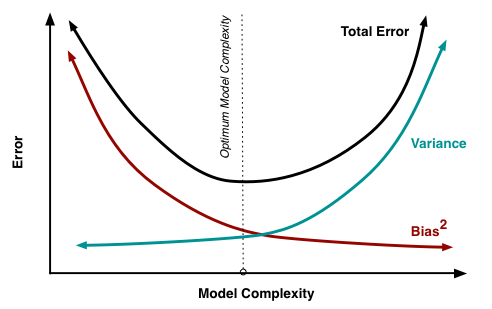
\includegraphics[ width=0.5\textwidth]{BiasVariance}
	\caption[Bias-Varianza trade-off]{\textit{Bias-Varianza trade-off}}
   \label{fig:bvtrd}
\end{figure}

\section[Tecniche selezione class.]{Model selection,Model evaluation,algorithm selection}
Il workflow nella creazione di un classificatore che funga da predittore per un problema di classificazione supervisionato è tipicamente il seguente:
\begin{description}
\item[\textbf{Algorithm selection}] E' necessario scegliere il modello\footnote{Malgrado in letteratura si parli di selezione dell'algoritmo e più corretto parlare di selezione di un modello perchè, ad esempio in un modello come \ac{SVM} l'algoritmo rappresenta la specifica tecnica risolutiva utilizzata per affrontare il problema matematico delineato da \ac{SVM}}. Spesso conoscendo pregi e difetti dei vari modelli la selezione avviene manualmente a secondo del modello che sembra più cofacente al problema da risolvere. E' possibile tuttavia effettuare la selezione usando delle tecniche per comparare i vari modelli tra di loro per stabilire quale esibisce le migliori perfomances in base a qualche misura.
\item[\textbf{Model selection}] Con l'intento di migliorare le perfomances di generalizzazione è necessario scegliere ,a partire dal \textit{training set}, il classificatore\footnote{Malgrado in letteratura si parli di model selection è un classificatore che va selezionato.} con le migliori performances, in base a qualche misura , dallo spazio delle ipotesi. A tal fine  i modelli hanno uno o più \textit{iperparametri} cioè delle manopole da regolare.
\item[\textbf{Model evaluation}] Si vogliono stimare le performances di generalizzazione, le performances predittive (in base a qualche misura) del nostro classificatore basandoci sul \textit{test set}.
\end{description}
Per raggiungere gli obbiettivi suddetti diventa fondamentale stabilire una misura da utilizzare. Nella sezione \ref{sub:measure} vi è una breve panoramica delle misure più note che si possono adottare.

\subsection{Holdout}
\label{sub:hol}
Questa è una delle tecniche più semplici ma anche efficaci. Si parte dal caso semplice nel quale si vuole fare solo model evaluation e già si conoscono i parametri migliori e quindi non è neccessario fare model selection. Il principio ispiratore è che fare l'addestramento del classificatore e la sua valutazione sullo stesso insieme produce un'accuracy ottimisticamente biased. \textbf{Holdout} divide i campioni disponibili in un \textit{training set} e un \textit{test set} in maniera casuale di solito in maniera 2/3 1/3. Si fa l'addestramento sul \textit{training set} e poi il classificatore ottenuto viene valutato sul \textit{test set}. Infine si rieffettua l'addestramento su tutti i campioni inizialmente disponibili\footnote{Riaddestrare alla fine del processo su tutti i campioni possibili è una tecnica valida solo se si è adottata la stratificazione(vedasi \ref{stra:stra}) nello splitting dei campioni iniziali,perchè assicura che i campioni nei vari insiemi splittati restino statisticamente indipendenti}. Questo metodo ha due grandi limiti:
\begin{enumerate}
\item La suddivisone casuale dei campioni in holdout può alterare le proprietà statistiche dei campioni. Questi sono assunti essere estratti dalla stessa distribuzione di probabilità ed essere statisticamente indipendenti. Questa proprietà può venire meno: ad esempio partendo da campioni bilanciati si potrebbero generare \textit{training set} e \textit{test set} non bilanciati.
\item \label{item:holdlim} Utilizzare un numero ridotto di campioni (2/3) per effettuare l'addestramento può produrre una stima delle performances pessimisticamente biased. Si ha cioè che il classificatore non ha ancora raggiunto la sua capacità e si potrebbe apprendere un classificatore migliore utilizzando un numero di campioni più grande. 
\end{enumerate}
Il primo problema può essere superato usando una tecnica chiamata
\label{stra:stra} \textbf{stratificazione} che consiste nel suddividere l'insieme di campioni iniziale in due insiemi in modo che il bilanciamento delle classi di campioni con diverse etichette sia ancora rispettato nei risultanti sottoinsiemi. Il secondo problema invece è strutturale in quanto se si usassero tutti i campioni disponibili per l'addestramento poi si dovrebbero valutare le performances su questi stessi campioni producendo stime ottimisticamente biased. Inoltre lo scenario tipico è quello in cui si vuole fare sia model selection che model evaluation. In quest ultimo caso è necessario dividere l'insieme di campioni di partenza in (usando la stratificazione):
\begin{itemize}
\item \textbf{un training set}
\item \textbf{un validation set}
\item \textbf{un test set}
\end{itemize} 
Prima si fa model selection effettuando l'addestramento sul \textit{training set} nello spazio dei parametri. Ad esempio se si usa una tecnica come \textbf{grid-search} per ogni parametro vanno scelti i valori oppure il range in cui i valori possono variare e il passo di variazione e poi si deve effettuare l'addestramento per ogni istanza dei parametri. Alla fine ognuno di questi classificatori va valutato in base a qualche misura sui campioni del \textit{validation set} e si seleziona il modello che massimizza tale misura. Quindi in questo modo si scelgono gli iperparametri migliori. A questo punto si rieffettua l'addestramento del classificatore risultato migliore usando sia i campioni del \textit{training set} che quelli del \textit{validation set}. A questo punto si fa model evaluation, cioè il classificatore ottenuto viene valutato sul \textit{test set}. Alla fine si riaddestra su tutti i campioni inizialmente disponibili (con l'istanza di parametri trovata). Avendo usato in fase di model evaluation un classificatore addestrato con meno campioni(\textit{training set} e \textit{validation set}) di quelli totali è molto probabile che le misure rilevate siano delle stime pessimisticamente biased. 

\subsection{Validazione incrociata}
Con la \textit{cross validation} (validazione incrociata) si supera il limite di holdout che è quello di produrre delle stime pessimisticamente biased. Il principio di funzionamento si basa sulla constatazione che usare un numero di campioni maggiore per l'addestramento tendenzialmente fa diminuire la varianza e anche il bias. Occorre sottolineare che con questa tecnica non otteniamo un predittore ma una misura della qualità del predittore nel generalizzare. Ne esistono molte varianti, una delle più note è \textbf{k-fold-validation} che consiste nel suddividere l'insieme di campioni in k folds (cioè insiemi) ed addestrare un classificatore  sui campioni di k-1 folds ed usare il restante fold per effettuare la validazione ottenendo una misura d'accuracy. Poi si rifà la stessa cosa usando però un altro insieme di validazione riaddestrando un predittore sugli altri k-1 folds. E così via finchè tutti i k folds vengono usati esattamente una volta come insieme di validazione. Infine si fa la media dei k indici di errore ricavati(sono i valori di accuracy)  ottenendo una stima della capacità di generalizzare. In questo modo si fanno k addestramenti. L'idea principale che vi sta dietro è che tutti gli elementi dell'insieme hanno l'opportunità di essere testati producendo una misura più attendibile. Un'altra tecnica è \textbf{LOO(Leave-one-out cross-validation)} che è uguale a k-fold-validation con k pari alla dimensione dell'insieme quindi l'insieme di validazione di volta in volta sarà composto da un solo elemento ma sarà necessario fare un numero di addestramenti pari al numero di campioni nell'insieme. LOO è da preferire quando l'insieme è particolarmente piccolo. LOO è quasi unbiased quindi ha un bias pessimistico anche minore di k-fold-validation ma esibisce una più grande varianza. Aumentando k il bias decresce (più accurato),la varianza aumenta (più variabilità), il costo computazionale aumenta.\\Quindi dovendo fare model selection e model evaluation si suddividono i campioni iniziali in un \textit{training set} e un \textit{test set} (usando la stratificazione) e poi si applica k-fold-validation sul \textit{training set} su ogni istanza degli iperparametri (usando grid-search ad esempio)  e si seleziona il migliore classificatore (k-fold-validation assicura una misura più attendibile e quindi una scelta dei parametri e di conseguenza del classificatore presumibilmente migliore). In seguito si effettua l'addestramento sull'intero \textit{training set} con gli iperparametri precedentemente ottenuti e si valuta il classificatore sul \textit{test set}(in quest ultimo step di solito non si usa l'accuracy ma una delle misure descritte nella \ref{sub:measure} ad esempio). In ultima analisi si effettua un addestramento su tutti i campioni inizialmente disponibili(\textit{training set} e \textit{test set}). 

\subsection{Algorithm selection}
Oltre che la selezione del classificatore è possibile anche stabilire quale sia il modello più adatto per un problema specifico in maniera oggettiva. Queste tecniche non sono molto utilizzate perchè spesso è il progettista che sceglie un modello piuttosto che un altro in anticipo, scegliendo in base alle caratteristiche del problema stesso il modello che sembra più idoneo. Ed in questa tesi è stato questo il caso dato che si è scelto di usare \ac{SVM} quindi questa sottosezione non sarà approfondita più di tanto. Qui si precisa che si è optato per quest'ultima opzione in quanto il confronto dei vari modelli ne comporta comunque l'implementazione del modello per il problema in questione quindi avrebbe  comportato un notevole sforzo implementativo. In questa sede si menziona solo che una delle tecniche più note in tal senso è \textbf{nested-cross-validation}.

\subsection{Boosting}
\label{sub:boost}
Esistono delle tecniche alternative che si basano sulla combinazione di classificatori e propongono di addestrare $T$ classificatori diversi per lo stesso problema e di combinare i risultati. In generale la combinazione di classificatori ,si applica a problemi ritenuti difficili che danno risultati non soddisfacenti con le tecniche classiche, al fine di ridurre il rischio di \textit{overfitting}. Una di queste tecniche è il \textbf{boosting} ,il cui obiettivo principale è ridurre il bias,  che si basa sull'addestramento sequenziale di un certo numero di classificatori detti deboli  che combinati insieme producono un classificatore forte \footnote{Per classificatore debole e forte si intende rispettivamente con scarsa capacità di generalizzare (accuracy leggermente superiore al 50\%) e con ottime capacità di generalizzazione}. Per capirne in dettaglio il funzionamento si porta l'esempio di uno degli algoritmi di boosting più noto: AdaBoost descritto per la classificazione binaria. Ogni campione del training set ha un peso $w$ e quei campioni classificati  dai classificatori precedenti in modo errato avranno un peso maggiore (al primo passo i pesi sono assunti uniformi, ad esempio tutti pari ad $1/l$). Ad ogni passo $t$ si seleziona il classificatore $h_t$ che riduce l'errore pesato sui campioni del \textit{training set} cioè che minimizza:
\begin{equation*}
\epsilon_t = \sum_{\substack{i=1 \\ h_{t}(x_{i}) \neq y_{i}}}^{l}w_{i,t}
\end{equation*}
 Poi si calcola il peso da usare per il classificatore corrente come $\alpha_t = \frac{1}{2}\ln \bigl(\frac{1-\epsilon_t}{\epsilon_t}\bigl)$. Invece i pesi per il \textit{training set} da utilizzare al passo successivo a partire dai pesi al passo corrente si otterrano come:
 \begin{equation*}
 w_{i,t+1} = w_{i,t}e^{-y_{i}h_{t}(x_{i})}
 \end{equation*}
Assumendo di usare $T$ classificatori deboli il classificatore forte $H_T$ e la classificazione di un campione del \textit{test set} x, si ottengono come:
\begin{equation*}
H_{T}(x) = sign\Biggl(\sum_{i=1}^{T}\alpha_ih_i(x)\Biggl)
\end{equation*}

\section{Data Preprocessing}
Nella maggior parte dei casi i campioni grezzi in input non possono essere usati direttamente. I campioni vanno manipolati al fine di avere delle migliori performances o perchè i campioni sono composti da attributi (gli attributi sono le singole componenti dei campioni) categorici ed il modello presuppone in ingresso attributi numeri. 
\subsection{Codifiche}
L'esigenza di adottare una codifica dei campioni deriva quasi sempre dal fatto che il modello adottato richiede in ingresso attributi numerici invece i campioni si compongono di attributi categorici\footnote{Un esempio di attributo categorico è un componente di un campione che può assumere solo i valori rosso,verde,giallo}. Qui si descrivono due tipi di codifiche.
\subsubsection{Integer Encoding}
\label{subsub:ien} 
Per ogni attributo categorico di ogni campione, si associa una specifica categoria ad un numero dell'insieme $\mathbb{N}$.
Ad esempio per l'attributo categorico che rappresenta i colori del semaforo una possibile codifica è:
\begin{alignat}{3}
&verde \to 0 \\
&giallo \to 1\\
&rosso \to 2
\end{alignat} 
In questo modo il campione $\Braket{verde , 9}$ che è composto da due attributi che indicano il colore del semaforo e l'ora viene codificato come $\Braket{0 , 9}$ e si osservi che il secondo attributo essendo già numerico non viene codificato.
\subsubsection{One Hot Encoding}
\label{subsub:ohe}
\ac{OHE} (One Hot Encoding) assegna un bit ad ogni classe di un attributo. La lunghezza di questa codifica è quindi il numero di classi dell' attributo. Riproponendo l'esempio della sottosezione \ref{subsub:ien} una possibile codifica per le classi dell'attributo categorico semaforo è:
\begin{alignat}{3}
&verde \to 0 0 1\\
&giallo \to 0 1 0\\
&rosso \to 1 0 0
\end{alignat}
Se il numero di classi non è troppo grande questa codifica può essere più stabile rispetto a \textit{integer encoding}.  
Nel caso di campioni codificati con \ac{OHE} non è necessario fare lo \textbf{scaling} o la \textbf{normalizzazione} (sottosezione \ref{subsub:scal}).

\subsection{Scaling}
\label{subsub:scal}
Lo \textbf{scaling} o \textbf{normalizzazione} si rende necessaria quando esistono attributi che variano in un range di valori molto diversi gli uni dagli altri. Infatti se si usa un modello che calcola una distanza, come la distanza euclidea, tra i campioni si ha che l'attributo che ha i valori più grandi domina questa misura rendendo ininfluente il contributo degli altri attributi. Per evitare che ciò avvenga si può riscalare il range degli attributi in modo che varino in [0,1] o in [-1,1]. Lo scaling va effettuato per tutti gli attributi ma procedendo per singolo attributo: sia x il vettore associato a uno specifico attributo formato dal valore per quell attributo di tutti i campioni del \textit{training set}, si ha che un possibile vettore normalizzato $x'$ in [0 1] si ottiene con:
\begin{equation*}
x' = \frac{x - min(x)}{max(x) - min(x)}
\end{equation*}  
Questo calcolo va effettuato per tutti gli attributi.
Un'altra tecnica di scaling è la \textbf{standardizzazione} che  calcola la media $\overline{x}$ e la deviazione standard $\sigma$ del vettore attributo x ed ottiene il vettore standardizzato $x'$ come:
\begin{equation}
\label{eq:stand}
x' = \frac{x - \overline{x}}{\sigma}
\end{equation}  
$x'$ sarà a media zero e a varianza unitaria. Questo calcolo va effettutato per ogni attributo.La standardizzazione riduce il range di variazione ma a differenza del precedente non assicura che i dati varino esattamente nel range [0 1] . Il pregio della standardizzazione consiste nel fatto che a differenza del primo metodo illustrato è in grado di gestire gli \textit{outliers} cioè un valore di un attributo molto grande rispetto agli altri valori dello stesso attributo.
In generale un altro vantaggio di effettuare lo scaling è che rende più veloci alcuni modelli come le \ac{SVM} ad esempio. Inoltre nel caso in cui i dati fossero precedentemente stati codificati con \ac{OHE} lo scaling non si effettua perchè gli attributi avranno valori binari(0 oppure 1 quindi valori già normalizzati).
Nei casi pratici per impedire di effettuare una divisione per zero quando la deviazione standard è nulla è necessario aggiungere un valore piccolo. Infine è molto importante scalare i campioni del \textit{test set} con gli stessi valori con cui sono stati scalati i campioni del \textit{training set} in altre parole per scalare il \textit{test set} si devono utilizzare gli stessi valori di media e varianza calcolati e salvati precedentemente per il \textit{training set}  invece che calcolarli dal \textit{test set}. 

\subsection{Feature extraction}
\textbf{Feature extraction} consiste nell'estrarre dai campioni delle \textit{features}, ossia delle informazioni rilevanti. In alcuni casi accade che i dati originali, o anche sottoposti a codifica o scaling, sono inappropriati per risolvere un determinato problema. In molti frangenti delineare delle \textit{features} idonee al problema consente di ottenere risultati migliori. Analogo è il concetto di \textit{feature selection} in cui una \textit{feature} diventa un sottoinsieme degli attributi originali, mentre in \textit{feature extraction} si applica una qualche trasformazione agli attributi selezionati.
Un altro vantaggio insito in questa tecnica è la diminuizione della dimensionalità dello spazio di input individuando e rimuovendo attributi non necessari o ridondanti. Ciò dovrebbe produrre dei modelli meno complessi ed aumentare l'accuracy del predittore.

\section{Addestrare una SVM}
\label{sec:adsvm}
Per incrementare le prestazioni del modello \ac{SVM} esistono delle regole d'oro che andrebbero seguite. Rifacendosi a \cite{SvmPracticalGuide10} e \cite{SvmAnotherPracticalGuide14} si ha che le linee guide per utilizzare le \ac{SVM} al meglio sono le seguenti:
\begin{description}
\item[Preprocessing dei campioni] \ac{SVM} esige che i campioni da presentare in ingresso siano sotto forma di vettori di numeri reali. Quindi è necessario effettuare:
\begin{itemize}
\item \textbf{Codifica} Nel caso di attributi categorici ad $m$ classi con $m$ piccolo è conveniente utilizzare una codifica come \ac{OHE} anzichè Integer Encoding. Integer Encoding può essere adottata nel caso in cui $m$ sia grande.
\item \textbf{Scaling} Lo scaling dei campioni è molto importante con \ac{SVM} non solo per i motivi delineati nella sottosezione \ref{subsub:scal} (che restano validi) ma anche perchè se si usano alcuni tipi di \textit{kernel}  come ad esempio il \textit{kernel polinomiale}  valori degli attributi molto grandi possono causare dei problemi numerici (il risultato del prodotto scalare di questo \textit{kernels} produrrà valori troppo grandi per essere rappresentati correttamente). Allora si effettua  una normalizzazione nel range [-1 1] o [0 1] oppure una standardizzazione. Si osservi che \textit{kernels} come quello gaussiano sono già normalizzati cioè variano automaticamente in un range predefinito ed in questi casi vengono a cadere i problemi numerici e tecniche come la standardizzazione, nonostante non garantiscono a priori un range prefissato , possono essere convenientemente utilizzate (per impedire che gli attributi che varino in un range più grande dominino gli attributi che varino in un range più piccolo). Se è avvenuta una precedente codifica come \ac{OHE} lo scaling non si applica.
\end{itemize}
\item[Model selection] Nel caso in cui la dimensionalità dei campioni sia molto grande oppure si è applicato un \textit{kernel} che si spera renda i campioni linearmente separabili si potrebbe sperare di usare con fiducia hard margin anche se come detto nell'appendice \ref{cap:cinque} è spesso consigliabile scegliere comunque soft margin. Si ha quindi che $C$ è un parametro spesso presente anche con dati linearmente separabili. Inoltre si ha che prima di utilizzare un \textit{kernel} adatto a un problema specifico si prova uno di quelli predefiniti e in questo caso la scelta ricade spesso sul \textit{kernel} gaussiano perchè quello sigmoidale  rispetta le condizioni di Mercer solo per alcuni valori dei parametri e si dimostra che per alcuni valori dei parametri diventa un sottocaso del \textit{kernel gaussiano}, e quello polinomiale consta di due o tre parametri a dispetto di un parametro nel gaussiano, e anche perchè come detto il \textit{kernel} gaussiano è automaticamente normalizzato e non presenta difficoltà numeriche e tra quelli predefiniti si è dimostrato esibire spesso performances migliori. Quindi il \textit{kernel gaussiano} è di solito consigliato come prima scelta per poi passare a \textit{kernel} ``ad hoc'' in caso di risultati insoddisfacenti. Un possibile modo di procedere è il seguente:
\begin{itemize}
\item \textbf{Validazione incrociata} Tipicamente si procede dividendo l'insieme di campioni processato (codifica o scaling)  in un \textit{un training set} e un \textit{test set}. Si effettua la validazione incrociata, tipicamente 5-fold-validation o 10-fold-validation , sul \textit{training set}. In questo modo si fa model selection ottenendo un classificatore (e quindi gli iperparametri) che esibisce una accuracy maggiore. Infine si fa \textbf{model evaluation} sul \textit{test set} per ottenere una qualche misura e poi si riaddestra \ac{SVM} sull'intero insieme di campioni iniziale  
\item \textbf{Grid-search} Nella procedura descritta immediatamente sopra è necessario scegliere un metodo per la selezione del classificatore migliore nello step di validazione incrociata. La possibilità più semplice è quella di utilizzare grid-search tuttavia esistono tecniche avanzate che ritornano una stima dell'accuracy della \textit{cross-validation}. Tuttavia quando è possibile (cioè sufficienti risorse computazionali) è preferibile sempre utilizzare grid-search che è una tecnica esaustiva che da una maggiore affidabilità. Inoltre si ha che la grid-search può essere parallelizzata per incrementare le prestazioni. Inoltre utilizzando il \textit{kernel} gaussiano si hanno solo due parametri  $C \text{ e } \gamma$ e quindi lo spazio di ricerca dei parametri non è eccessivamente ampio. Una scelta usuale per entrambi i parametri è di scegliere un passo esponenziale. Tipici intervalli sono $C = 2^{-5},2^{-3},\dots,2^{15}$  e $\gamma = 2^{-15},2^{-13},\dots,2^{3}$
\end{itemize}
\end{description}


\section{Misure}
\label{sub:measure}
Per un problema di classificazione binaria è possibile definire la matrice di confusione come in figura \ref{fig:mco} che stabilisce le seguenti quantità numeriche per un predittore binario:
\begin{description}
\item[TP(true positive)] Campioni positivi predetti dal classificatore come positivi.
\item[TN(true negative)] Campioni negativi predetti dal classificatore come negativi.
\item[FP(false positive)] Campioni negativi predetti erroneamente dal classificatore come positivi.
\item[FN(false negative)] Campioni positivi predetti erroneamente dal classificatore come negativi.
\end{description}

\begin{figure}[htp]
	\centering
	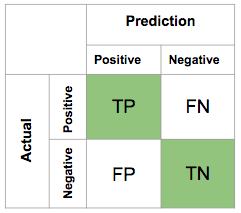
\includegraphics[ width=0.5\textwidth]{MatriceConfusione}
	\caption[Matrice di confusione]{\textit{Matrice di confusione per un problema di classificazione binaria}}
   \label{fig:mco}
\end{figure}

Allora si definisce l'\textbf{accuracy} come:
\begin{equation*}
Accuracy = \frac{TP + TN}{TP+TN+FP+FN}
\end{equation*}
e quindi indica la percentuale di campioni predetti correttamente rispetto alla totalità. Non è rilevante l'insieme su cui si definiscono la matrice di confusione e le varie misure, ad esempio è possibile calcolare l'accuracy sia sul \textit{training set} che sul \textit{test set}. Inoltre è possibile calcolare la percentuale d'errore facendo:
\begin{equation*}
Errore = 1 - Accuracy
\end{equation*}
 L'accuracy però non è una misura idonea per due ragioni:
 \begin{itemize}
 \item Se l'insieme su cui si calcola l'accuracy non è bilanciato la misura d'accuracy può essere ingannevole. Ad esempio immaginiamo che il  classificatore sia un \textit{majority class} che predice tutti i campioni come positivi e che il \textit{test set} abbia il 90\% di campioni positivi e i restanti negativi. In questo caso avremo un'accuracy pari a 0.9 cioè del 90\% nonostante il predittore sia pessimo.
 \item Anche se l'insieme fosse bilanciato, dall'accuracy non si evincerebbe se siano di più i FP oppure i FN, informazione che può essere rilevante.
 \end{itemize}
Per porre rimedio a questi problemi si usano \textbf{Precision (positive prediction value)} e \textbf{Recall (sensitivity o positive prediction value)} definite come:
\begin{alignat*}{2}
& Precision &= \frac{TP}{TP+FP}\\
& Recall &= \frac{TP}{TP+FN}
\end{alignat*}
Recall ci dice quanto è buono un classificatore nel predire i campioni positivi (in quanto avendo al denominatore tutti i dati positivi dell'insieme, Recall rappresenta la percentuale di campioni positivi predetta correttamente come tale). Un predittore \textit{majority class} che predice sempre i campioni come positivi (quindi FN=0) può ingannarci massimizzando Recall e rendendolo pari a 1. Precision ci dice quanti dei dati predetti come positivi sono positivi veramente; un predittore può essere ingannevole massimizzando quest'ultima misura se classifica come positivi i campioni dei quali ha una maggiore fiducia che siano positivi e negativi i restanti. Queste due misure non risultano comunque sufficienti nei casi, come questo lavoro, di \ac{IIR} da stringhe in cui risulta rilevante anche come vengono classificati i campioni negativi per cui si utilizzano altre due misure $Precision^{-}$(Negative prediction value) e $Recall^{-}$(Specificity o true negative rate) \cite{Bogdanov08} :
\begin{alignat*}{2}
& Precision^{-} &= \frac{TN}{TN+FN}\\
& Recall^{-} &=  \frac{TN}{TN+FP}
\end{alignat*} 
Queste ultime due misure hanno la stessa semantica di Precision e Recall ma sui campioni negativi. Si è accennato che le singole misure di per sè possono ancora essere ingannevoli tuttavia se combinate insieme tali problemi possono essere superati ad esempio se il predittore è un $majority class$ sempre positivo $Recall=1$ ma  $Recall^{-}=0$ (perchè TN=0) e quindi il problema può essere individuato. Inoltre utilizzare delle misure che combinano quelle definite sopra è necessario anche perchè per scegliere in maniera automatica un classificatore rispetto ad un altro è necessario avere un'unica misura. Uno dei criteri più noti e utilizzati è \textbf{F1-score (F-measure)} che effettua la media armonica tra Precisione e Recall quindi:
\begin{equation*}
\label{eq:f1s}
F1 = 2 \cdot \frac{Precision \cdot Recall}{Precision + Recall}
\end{equation*}
Questa misura può essere utilizzata in luogo dell'accuracy per insiemi non bilanciati tuttavia non fa ancora al caso nostro perchè non tiene conto dei campioni negativi che nel nostro scenario sono rilevanti. Una possibilità è quella di definire un F1-score anche sulla classe negativa usando la stessa equazione \eqref{eq:f1s} con $Precision^{-}\text{ e } Recall^{-}$ e poi mediare le due quantità, tuttavia in questo caso è più adatto e semplice utilizzare un'altra misura \textbf{MCC(Mattehws correlation coeffient)} definita come:
\begin{equation*}
MCC = \frac{TP \cdot TN−FP \cdot FN}{\sqrt{(TP+FP)(TP+FN)(TN+FP)(TN+FN)}}
 \end{equation*}
 Questa misura è ottima nel caso di dati non bilanciati e rappresenta bene la matrice di confusione ed è sicuramente più adatta di F1-score nel caso in cui sia i campioni positivi che quelli negativi sono rilevanti. Il valore ritornato varia tra $-1$ e $1$ e $0$ è equivalente ad un'accuracy del $50\%$.  Ad esempio un MCC di $0.5$ è comparabile ad un'accuracy del $75\%$. 